\documentclass[12pt, a4paper]{article}

% ─── Paquetes ────────────────────────────────────────────────────────────────
\usepackage{fontspec}
\usepackage[spanish]{babel}
\usepackage{geometry}
\usepackage{graphicx}
\usepackage{xcolor}
\usepackage{titlesec}
\usepackage{titletoc}
\usepackage{fancyhdr}
\usepackage{booktabs}
\usepackage{longtable}
\usepackage{array}
\usepackage{tabularx}
\usepackage{enumitem}
\usepackage{tcolorbox}
\usepackage{hyperref}
\usepackage{microtype}
\usepackage{parskip}
\usepackage{float}
\usepackage{caption}
\usepackage{subcaption}
\usepackage{mdframed}
\usepackage{multirow}
\usepackage{amsmath}
\usepackage{amssymb}

% ─── Geometría ───────────────────────────────────────────────────────────────
\geometry{
  top=2.5cm, bottom=2.5cm,
  left=2.8cm, right=2.8cm,
  headheight=15pt
}

% ─── Fuentes ─────────────────────────────────────────────────────────────────
\setmainfont{Helvetica Neue}[
  BoldFont = Helvetica Neue Bold,
  ItalicFont = Helvetica Neue Italic
]
\setsansfont{Helvetica Neue}
\setmonofont{Menlo}

% ─── Colores ─────────────────────────────────────────────────────────────────
\definecolor{primary}{HTML}{5B5CF0}
\definecolor{secondary}{HTML}{4A4BDB}
\definecolor{accent}{HTML}{EEF0FF}
\definecolor{darkgray}{HTML}{374151}
\definecolor{medgray}{HTML}{6B7280}
\definecolor{lightgray}{HTML}{F3F4F6}
\definecolor{bordergray}{HTML}{E5E7EB}
\definecolor{success}{HTML}{10B981}
\definecolor{warning}{HTML}{F59E0B}
\definecolor{danger}{HTML}{EF4444}
\definecolor{admincolor}{HTML}{7C3AED}
\definecolor{leadercolor}{HTML}{0369A1}
\definecolor{executorcolor}{HTML}{065F46}

% ─── Hyperref ────────────────────────────────────────────────────────────────
\hypersetup{
  colorlinks = true,
  linkcolor  = primary,
  urlcolor   = primary,
  citecolor  = primary,
  pdftitle   = {TaskFlow - Manual de Usuario},
  pdfauthor  = {Jota Emilio Lopez Ramirez y Esmeralda Rivas Guzmán},
  pdfsubject = {Manual de Usuario v1.0}
}

% ─── Encabezados de sección ──────────────────────────────────────────────────
\titleformat{\section}
  {\Large\bfseries\color{primary}}
  {\thesection.}{0.6em}{}[{\color{bordergray}\titlerule[0.5pt]}]

\titleformat{\subsection}
  {\large\bfseries\color{darkgray}}
  {\thesubsection.}{0.5em}{}

\titleformat{\subsubsection}
  {\normalsize\bfseries\color{medgray}}
  {\thesubsubsection.}{0.4em}{}

\titlespacing*{\section}{0pt}{1.6em}{0.8em}
\titlespacing*{\subsection}{0pt}{1.2em}{0.5em}
\titlespacing*{\subsubsection}{0pt}{0.8em}{0.3em}

% ─── Cabecera y pie de página ────────────────────────────────────────────────
\pagestyle{fancy}
\fancyhf{}
\fancyhead[L]{\small\color{medgray}\textbf{TaskFlow} — Manual de Usuario}
\fancyhead[R]{\small\color{medgray}v1.0}
\fancyfoot[C]{\small\color{medgray}\thepage}
\renewcommand{\headrulewidth}{0.4pt}
\renewcommand{\headrule}{\color{bordergray}\hrule width\headwidth height\headrulewidth}
\renewcommand{\footrulewidth}{0pt}

% ─── Cajas de información ────────────────────────────────────────────────────
\tcbuselibrary{skins, breakable}

\newtcolorbox{infobox}[1][]{
  enhanced, breakable,
  colback=accent, colframe=primary,
  fonttitle=\bfseries\small\color{primary},
  title={#1},
  left=8pt, right=8pt, top=6pt, bottom=6pt,
  boxrule=0.6pt, arc=4pt
}

\newtcolorbox{warningbox}[1][]{
  enhanced, breakable,
  colback=yellow!8!white, colframe=warning,
  fonttitle=\bfseries\small\color{warning},
  title={#1},
  left=8pt, right=8pt, top=6pt, bottom=6pt,
  boxrule=0.6pt, arc=4pt
}

\newtcolorbox{notebox}{
  enhanced, breakable,
  colback=lightgray, colframe=bordergray,
  left=8pt, right=8pt, top=5pt, bottom=5pt,
  boxrule=0.5pt, arc=3pt
}

% ─── Tablas ──────────────────────────────────────────────────────────────────
\renewcommand{\arraystretch}{1.35}
\newcolumntype{L}[1]{>{\raggedright\arraybackslash}p{#1}}
\newcolumntype{C}[1]{>{\centering\arraybackslash}p{#1}}

% ─── Listas ──────────────────────────────────────────────────────────────────
\setlist[itemize]{leftmargin=1.5em, itemsep=2pt, topsep=4pt}
\setlist[enumerate]{leftmargin=1.8em, itemsep=2pt, topsep=4pt}

% ─── Imágenes ────────────────────────────────────────────────────────────────
\graphicspath{{docs/screenshots/}}
\captionsetup{font=small, labelfont={bf,color=medgray}, textfont={color=darkgray}}

% ─── Comandos personalizados ─────────────────────────────────────────────────
\newcommand{\rolbadge}[2]{%
  \colorbox{#1}{\color{white}\footnotesize\bfseries\,#2\,}%
}
\newcommand{\admin}{\rolbadge{admincolor}{ADMIN}}
\newcommand{\leader}{\rolbadge{leadercolor}{LÍDER}}
\newcommand{\executor}{\rolbadge{executorcolor}{EJECUTOR}}

\newcommand{\stepnum}[1]{%
  \tikz[baseline=(char.base)]\node[circle,fill=primary,text=white,
  inner sep=1.5pt,font=\footnotesize\bfseries](char){#1};%
}

% ═══════════════════════════════════════════════════════════════════════════════
%  DOCUMENTO
% ═══════════════════════════════════════════════════════════════════════════════
\begin{document}

% ─── PORTADA ─────────────────────────────────────────────────────────────────
\begin{titlepage}
  \pagecolor{primary}
  \color{white}
  \vspace*{2cm}
  \begin{center}
    {\fontsize{52}{60}\selectfont\bfseries TaskFlow}\\[0.5em]
    {\Large\color{white!80!primary} Plataforma de Gestión de Proyectos y Tareas}\\[3cm]

    {\Huge\bfseries Manual de Usuario}\\[0.8em]
    {\large\color{white!70!primary} Guía completa para todos los roles del sistema}\\[3cm]

    \begin{tabular}{rl}
      \textbf{Versión:}   & 1.0 \\[4pt]
      \textbf{Fecha:}     & Junio 2026 \\[4pt]
      \textbf{Autores:}   & Jota Emilio Lopez Ramirez \\
                           & Esmeralda Rivas Guzmán \\[4pt]
    \end{tabular}

    \vfill
    {\small\color{white!60!primary}
      Documento confidencial — Uso interno\\
      TaskFlow \textcopyright\ 2026
    }
  \end{center}
\end{titlepage}
\nopagecolor

% ─── TABLA DE CONTENIDO ──────────────────────────────────────────────────────
\newpage
\thispagestyle{empty}
{\color{primary}\rule{\textwidth}{2pt}}\\[0.4em]
{\Large\bfseries\color{primary} Tabla de Contenido}\\[0.2em]
{\color{bordergray}\rule{\textwidth}{0.5pt}}
\vspace{0.5em}
\tableofcontents
\newpage

% ═══════════════════════════════════════════════════════════════════════════════
\section{Introducción}

TaskFlow es una plataforma web para la \textbf{gestión integral de proyectos y tareas} que permite a los equipos de trabajo planificar, asignar, monitorear y controlar su actividad mediante un tablero Kanban interactivo.

\subsection{Descripción general}

El sistema centraliza la información de proyectos, tareas y colaboradores en una interfaz unificada, facilitando la comunicación y el seguimiento del progreso. Sus principales capacidades incluyen:

\begin{itemize}
  \item Organización visual del trabajo mediante tablero Kanban con fases personalizables.
  \item Registro y seguimiento del tiempo invertido en cada tarea.
  \item Sistema de comentarios con archivos adjuntos para la comunicación del equipo.
  \item Dashboards de progreso y distribución de carga laboral.
  \item Control de acceso granular según el rol del usuario.
\end{itemize}

\subsection{Roles del sistema}

TaskFlow define tres roles con distintos niveles de acceso y responsabilidad:

\begin{table}[H]
\centering
\begin{tabularx}{\textwidth}{C{2.2cm} L{4cm} L{7.5cm}}
\toprule
\textbf{Rol} & \textbf{Perfil} & \textbf{Responsabilidades principales} \\
\midrule
\admin & Administrador del sistema &
  Gestión completa de usuarios, proyectos, fases y tareas.
  Monitoreo general, cambio de roles y eliminación de registros. \\
\addlinespace
\leader & Líder de proyecto &
  Creación y configuración de proyectos. Asignación de miembros.
  Gestión de tareas y fases. Consulta de carga laboral. \\
\addlinespace
\executor & Ejecutor de tareas &
  Actualización del estado de sus tareas. Registro de tiempo trabajado.
  Publicación de comentarios y archivos adjuntos. \\
\bottomrule
\end{tabularx}
\caption{Roles disponibles en TaskFlow}
\end{table}

\begin{infobox}[Importante]
Cada módulo del sistema indica el rol mínimo requerido para acceder a su funcionalidad. Los accesos se validan tanto en el frontend como en el backend.
\end{infobox}

\subsection{Tecnologías utilizadas}

\begin{table}[H]
\centering
\begin{tabularx}{\textwidth}{L{3.5cm} L{4cm} L{6cm}}
\toprule
\textbf{Capa} & \textbf{Tecnología} & \textbf{Descripción} \\
\midrule
Frontend  & React 19 + Vite   & Interfaz de usuario reactiva \\
Estilos   & TailwindCSS       & Sistema de diseño utilitario \\
Backend   & Node.js + Express & API REST con autenticación JWT \\
ORM       & Prisma            & Acceso a base de datos con tipado \\
Base de datos & PostgreSQL 16 & Almacenamiento relacional \\
Contenedores & Docker Compose & Despliegue reproducible \\
\bottomrule
\end{tabularx}
\caption{Stack tecnológico de TaskFlow}
\end{table}

% ═══════════════════════════════════════════════════════════════════════════════
\section{Acceso al Sistema}

\subsection{Inicio de sesión}

Para ingresar a TaskFlow, el usuario debe autenticarse con sus credenciales corporativas.

\textbf{Pasos:}
\begin{enumerate}
  \item Abra el navegador y acceda a la URL de la aplicación.
  \item Ingrese su \textbf{correo electrónico} en el campo correspondiente.
  \item Ingrese su \textbf{contraseña}.
  \item Presione el botón \textbf{«Iniciar Sesión»}.
\end{enumerate}

\begin{figure}[H]
  \centering
  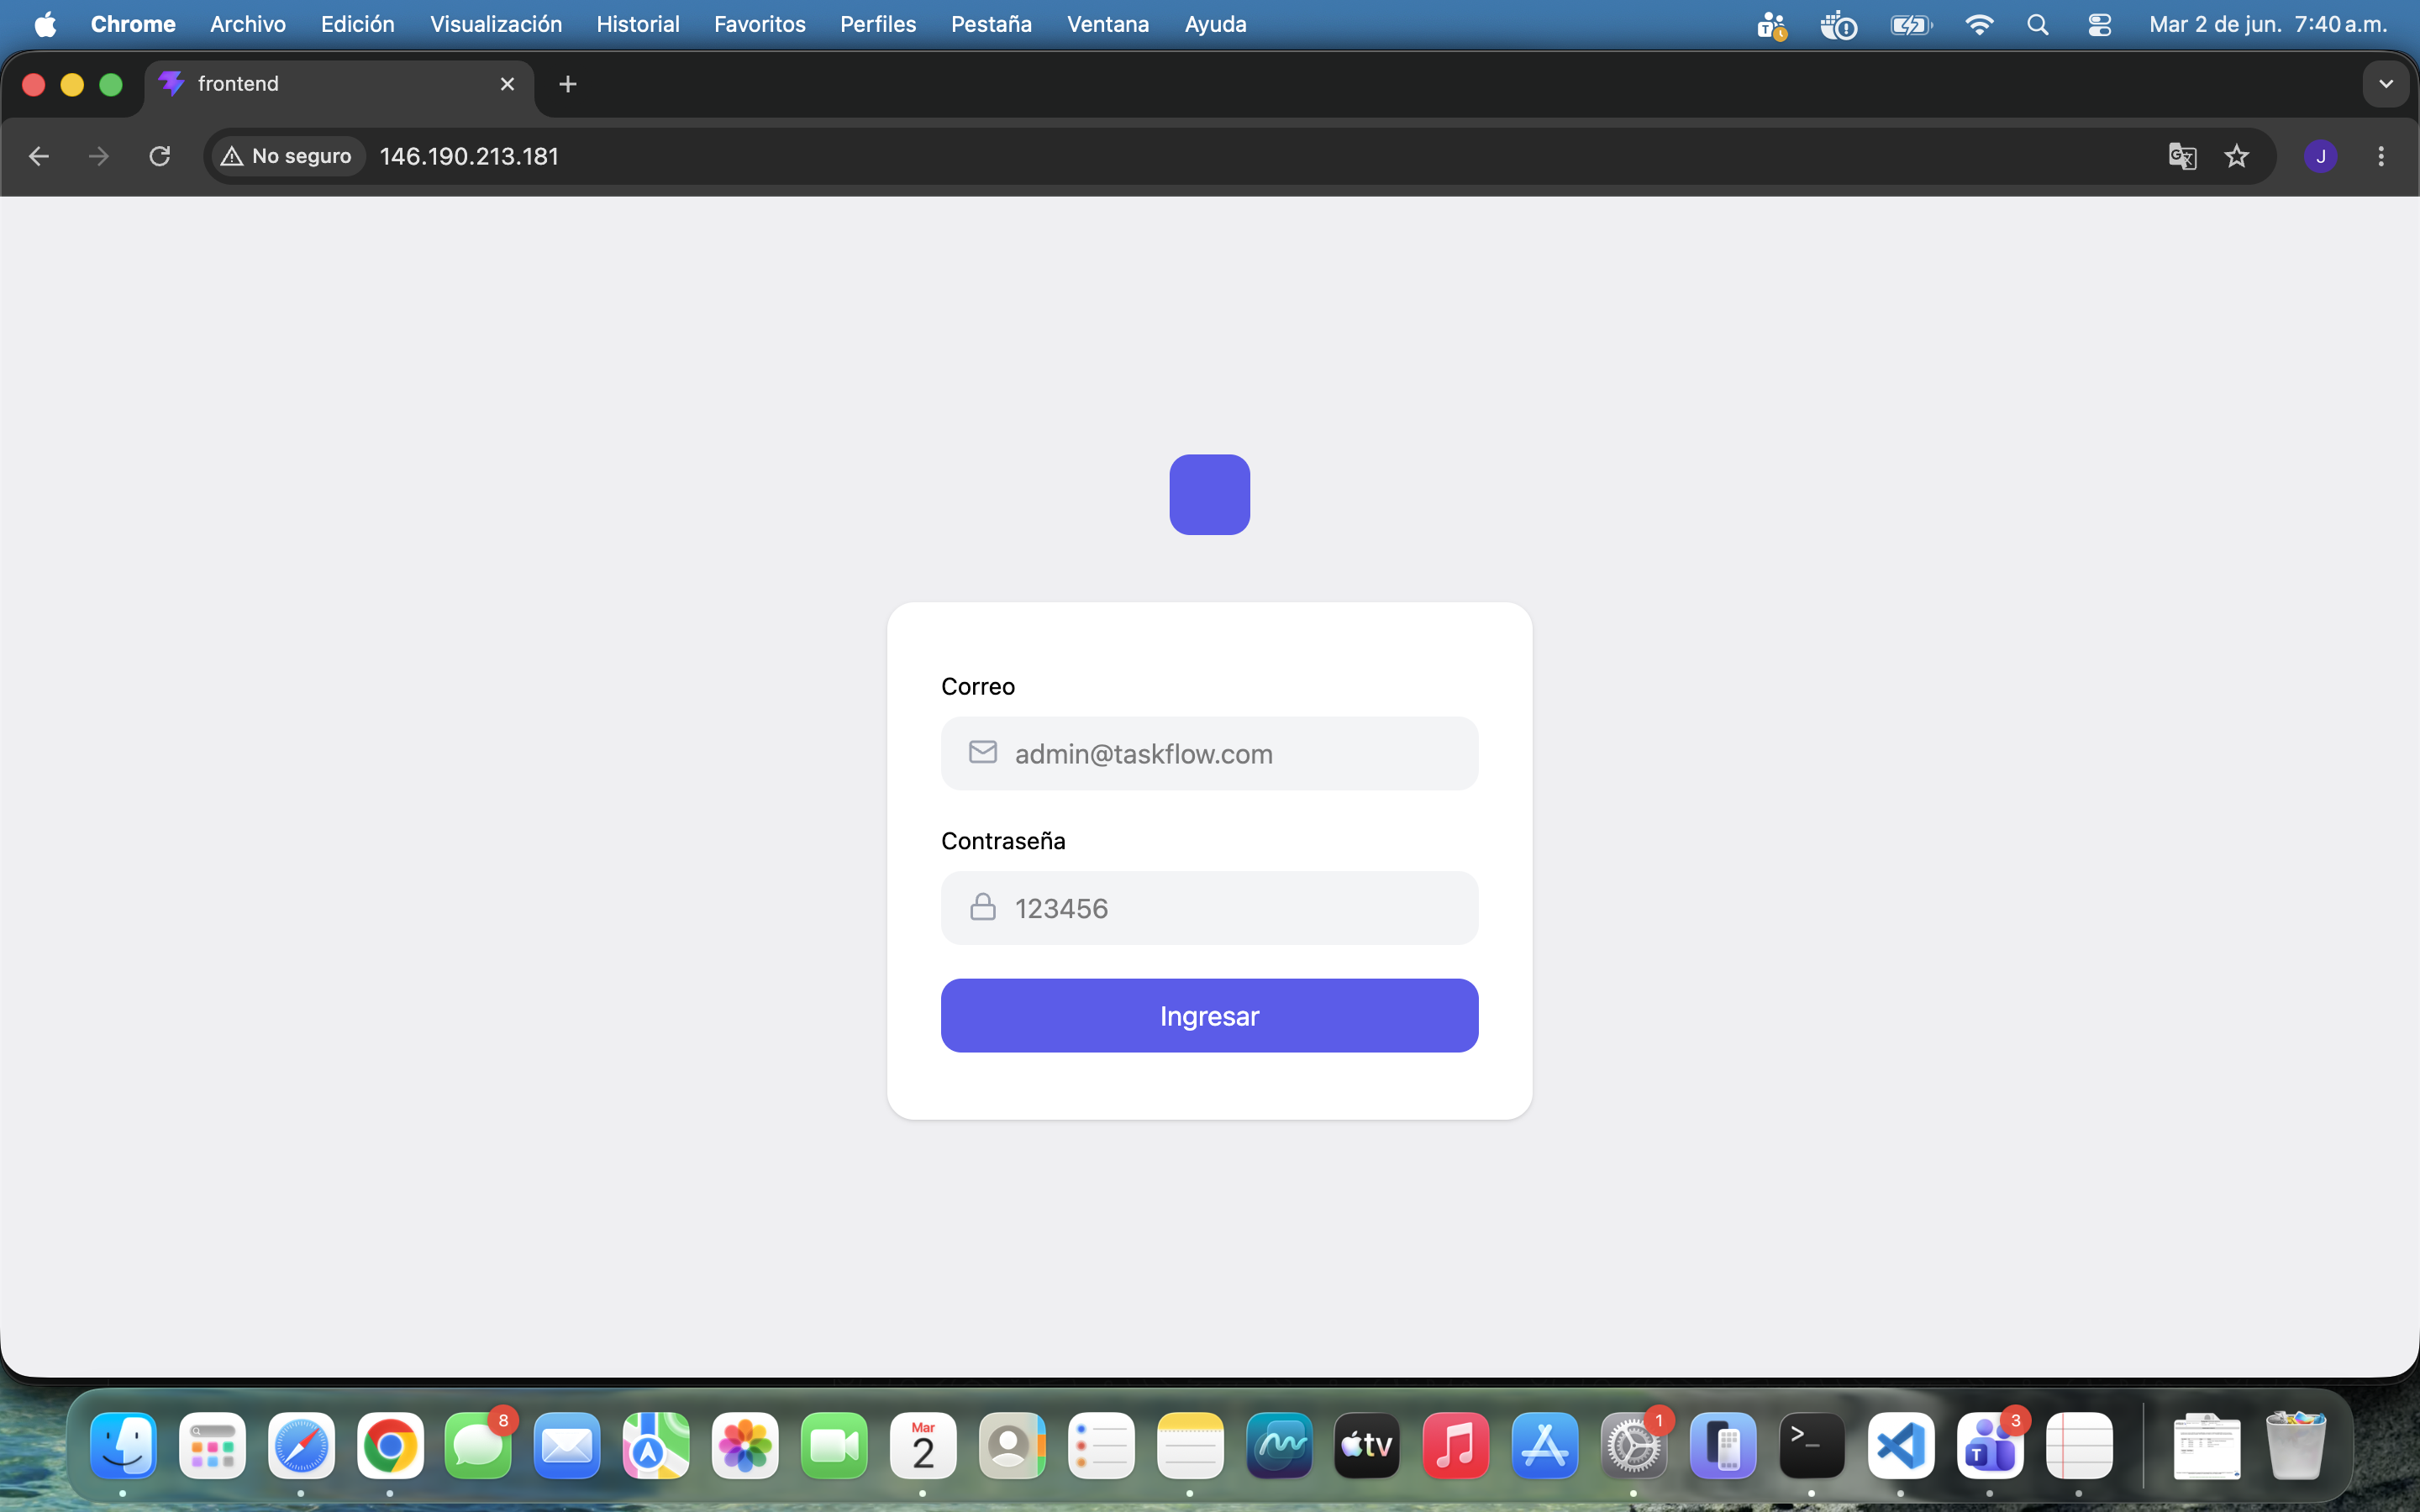
\includegraphics[width=0.75\textwidth]{login.png}
  \caption{Pantalla de inicio de sesión}
\end{figure}

\subsection{Resultado del acceso}

\begin{table}[H]
\centering
\begin{tabularx}{\textwidth}{L{4cm} L{9.5cm}}
\toprule
\textbf{Resultado} & \textbf{Descripción} \\
\midrule
Credenciales válidas &
  El sistema genera un token de sesión (válido por 8 horas) y redirige
  al usuario al panel principal adaptado a su rol. \\
\addlinespace
Credenciales inválidas &
  Aparece el mensaje \emph{«Credenciales inválidas»} y el usuario permanece
  en la pantalla de login. \\
\bottomrule
\end{tabularx}
\end{table}

\begin{warningbox}[Seguridad]
La sesión expira automáticamente después de 8 horas de inactividad. Si esto ocurre, el sistema lo redirigirá a la pantalla de login y deberá autenticarse nuevamente.
\end{warningbox}


% ═══════════════════════════════════════════════════════════════════════════════
\section{Página Principal (Home)}

\subsection{Panel principal}

Tras autenticarse, el usuario accede al panel principal que presenta una vista adaptada a su rol.

\begin{figure}[H]
  \centering
  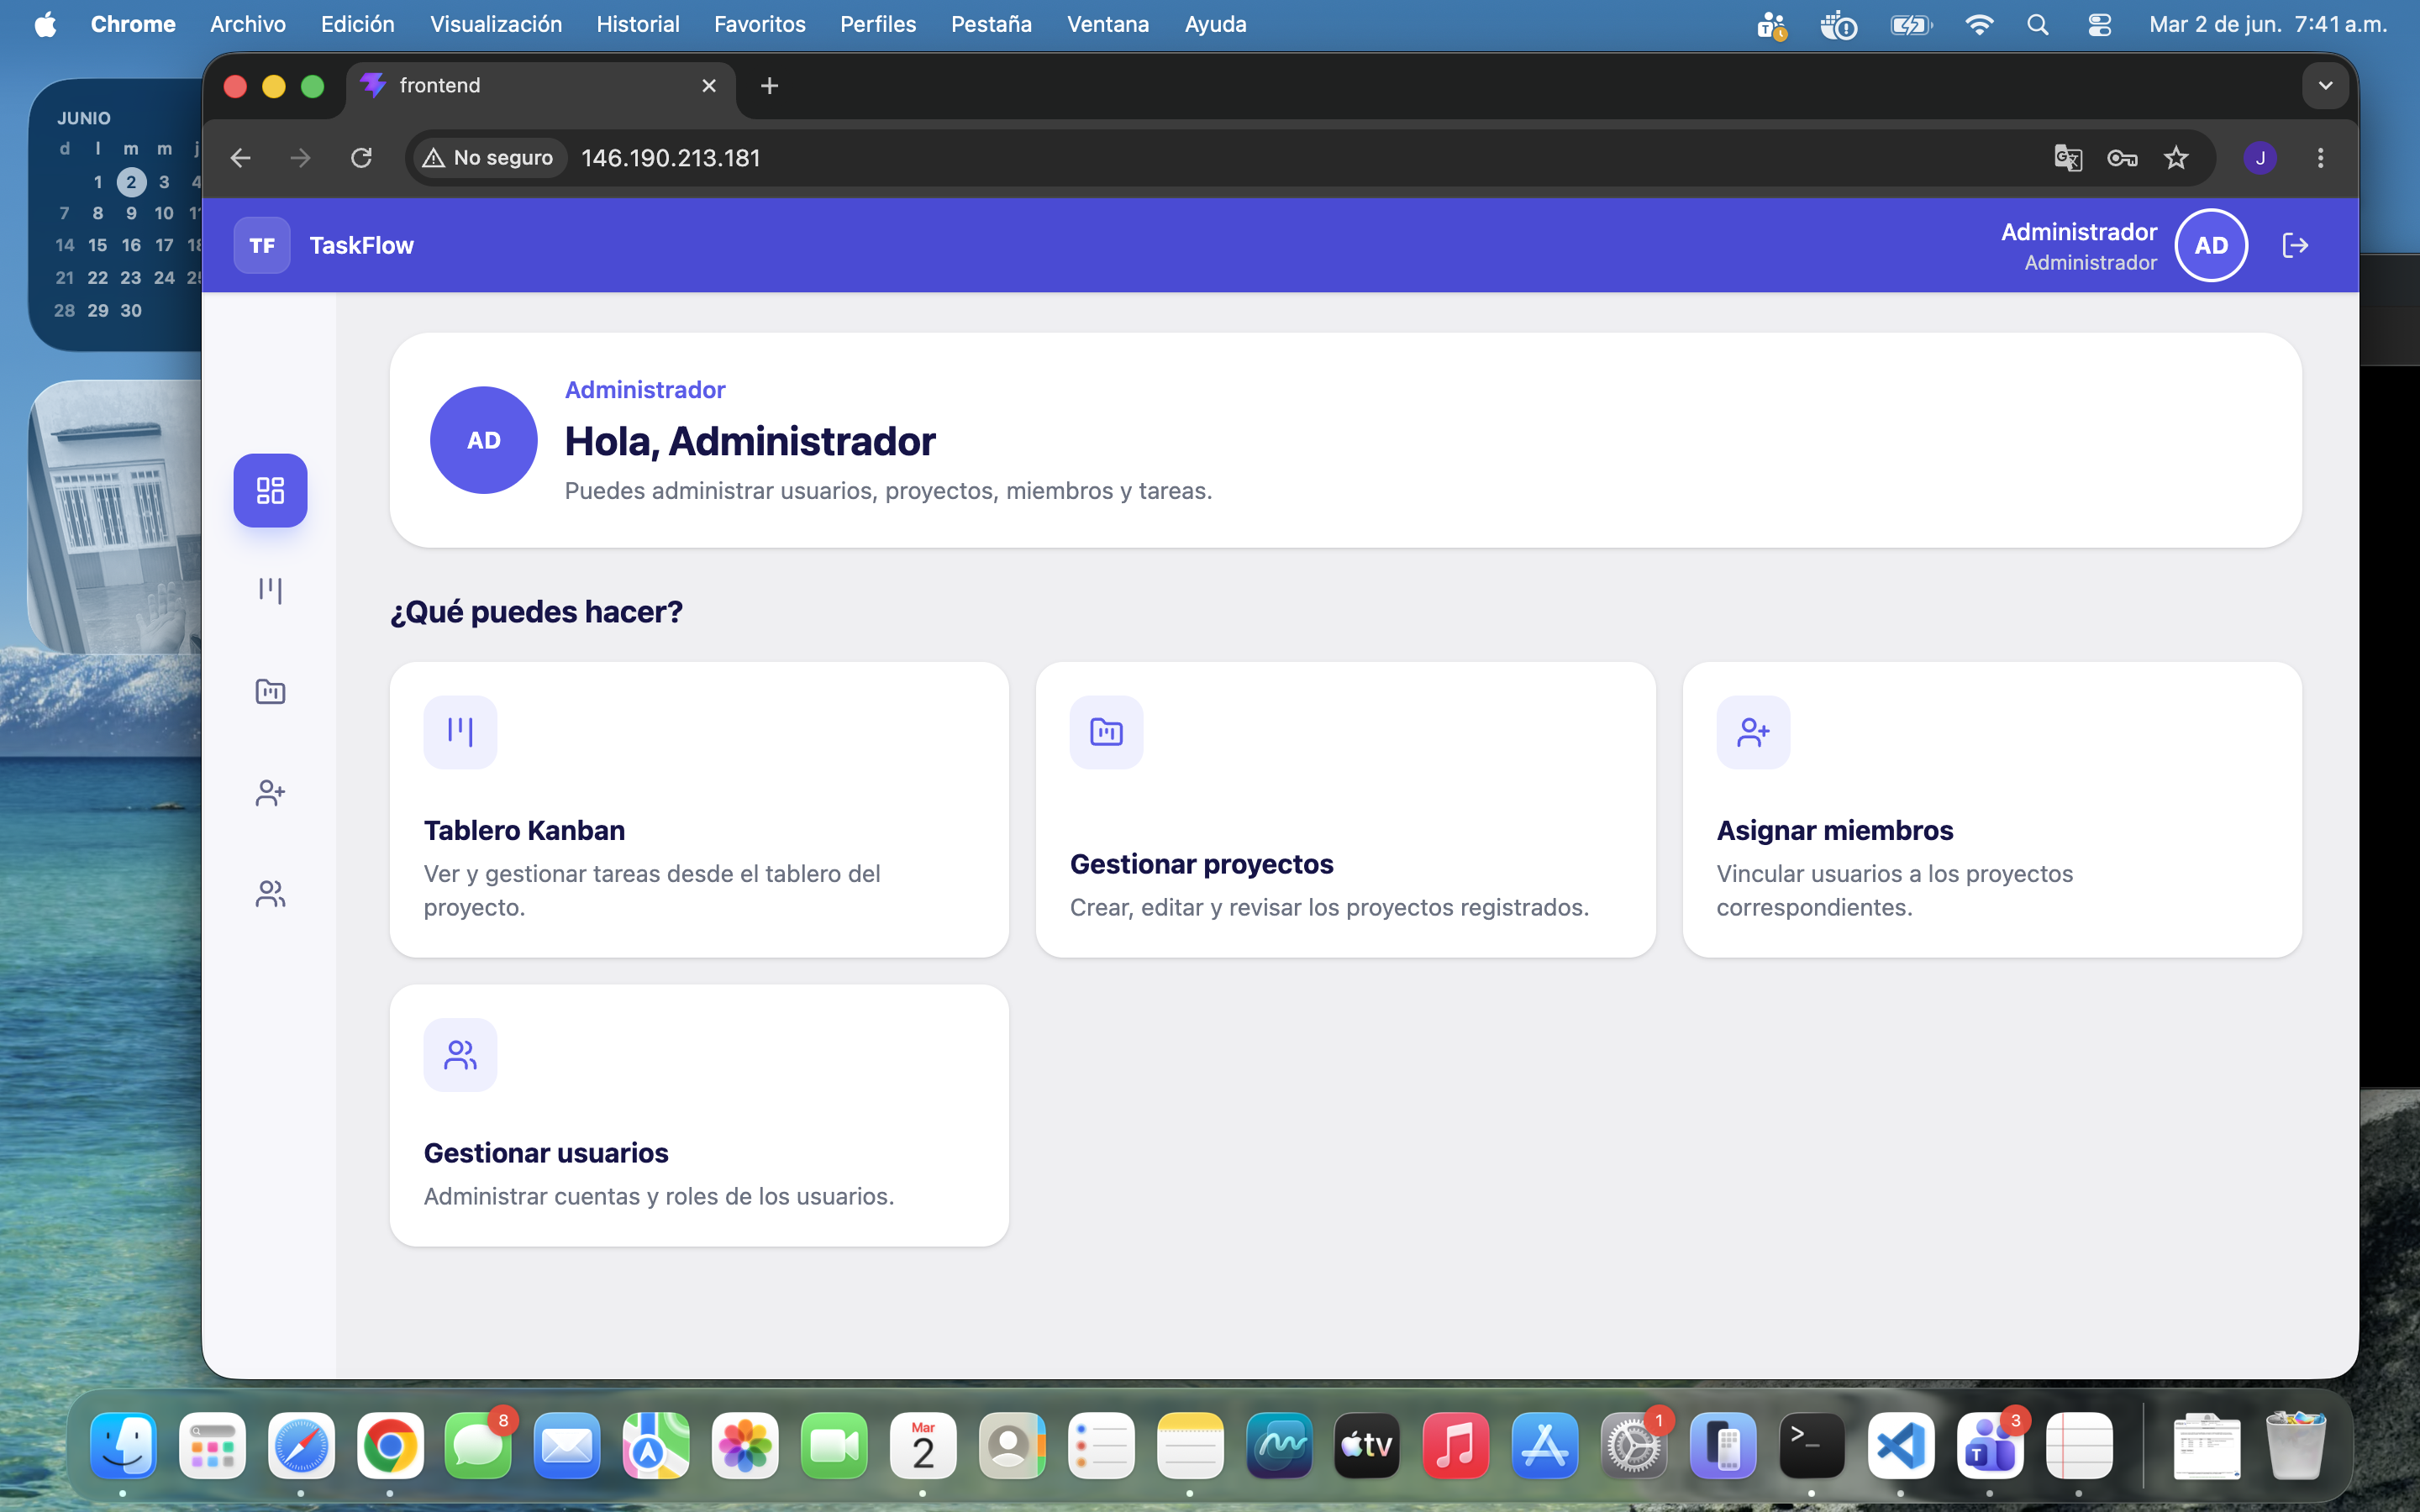
\includegraphics[width=0.90\textwidth]{home.png}
  \caption{Panel principal de TaskFlow}
\end{figure}

\subsection{Contenido según rol}

\begin{table}[H]
\centering
\begin{tabularx}{\textwidth}{L{2.5cm} L{11cm}}
\toprule
\textbf{Rol} & \textbf{Información y accesos disponibles} \\
\midrule
\admin &
  Acceso completo a todos los módulos: proyectos, tareas, usuarios, carga laboral y asignación de miembros. Indicadores generales del sistema. \\
\addlinespace
\leader &
  Acceso a proyectos en los que participa, tablero Kanban, miembros y carga laboral. No visualiza el módulo de usuarios. \\
\addlinespace
\executor &
  Acceso únicamente a los proyectos en los que ha sido incluido como miembro. Puede ver el tablero Kanban y las tareas que le corresponden. \\
\bottomrule
\end{tabularx}
\caption{Contenido del panel principal por rol}
\end{table}

\subsection{Navegación}

La barra lateral izquierda permite moverse entre los distintos módulos del sistema. Los módulos visibles varían según el rol del usuario autenticado.

% ═══════════════════════════════════════════════════════════════════════════════
\section{Gestión de Proyectos}

\begin{notebox}
\textbf{Roles con acceso:} \admin\ \leader
\end{notebox}

\subsection{Descripción}

El módulo de gestión de proyectos permite administrar el ciclo de vida completo de los proyectos: creación, configuración, seguimiento y eliminación.

\begin{figure}[H]
  \centering
  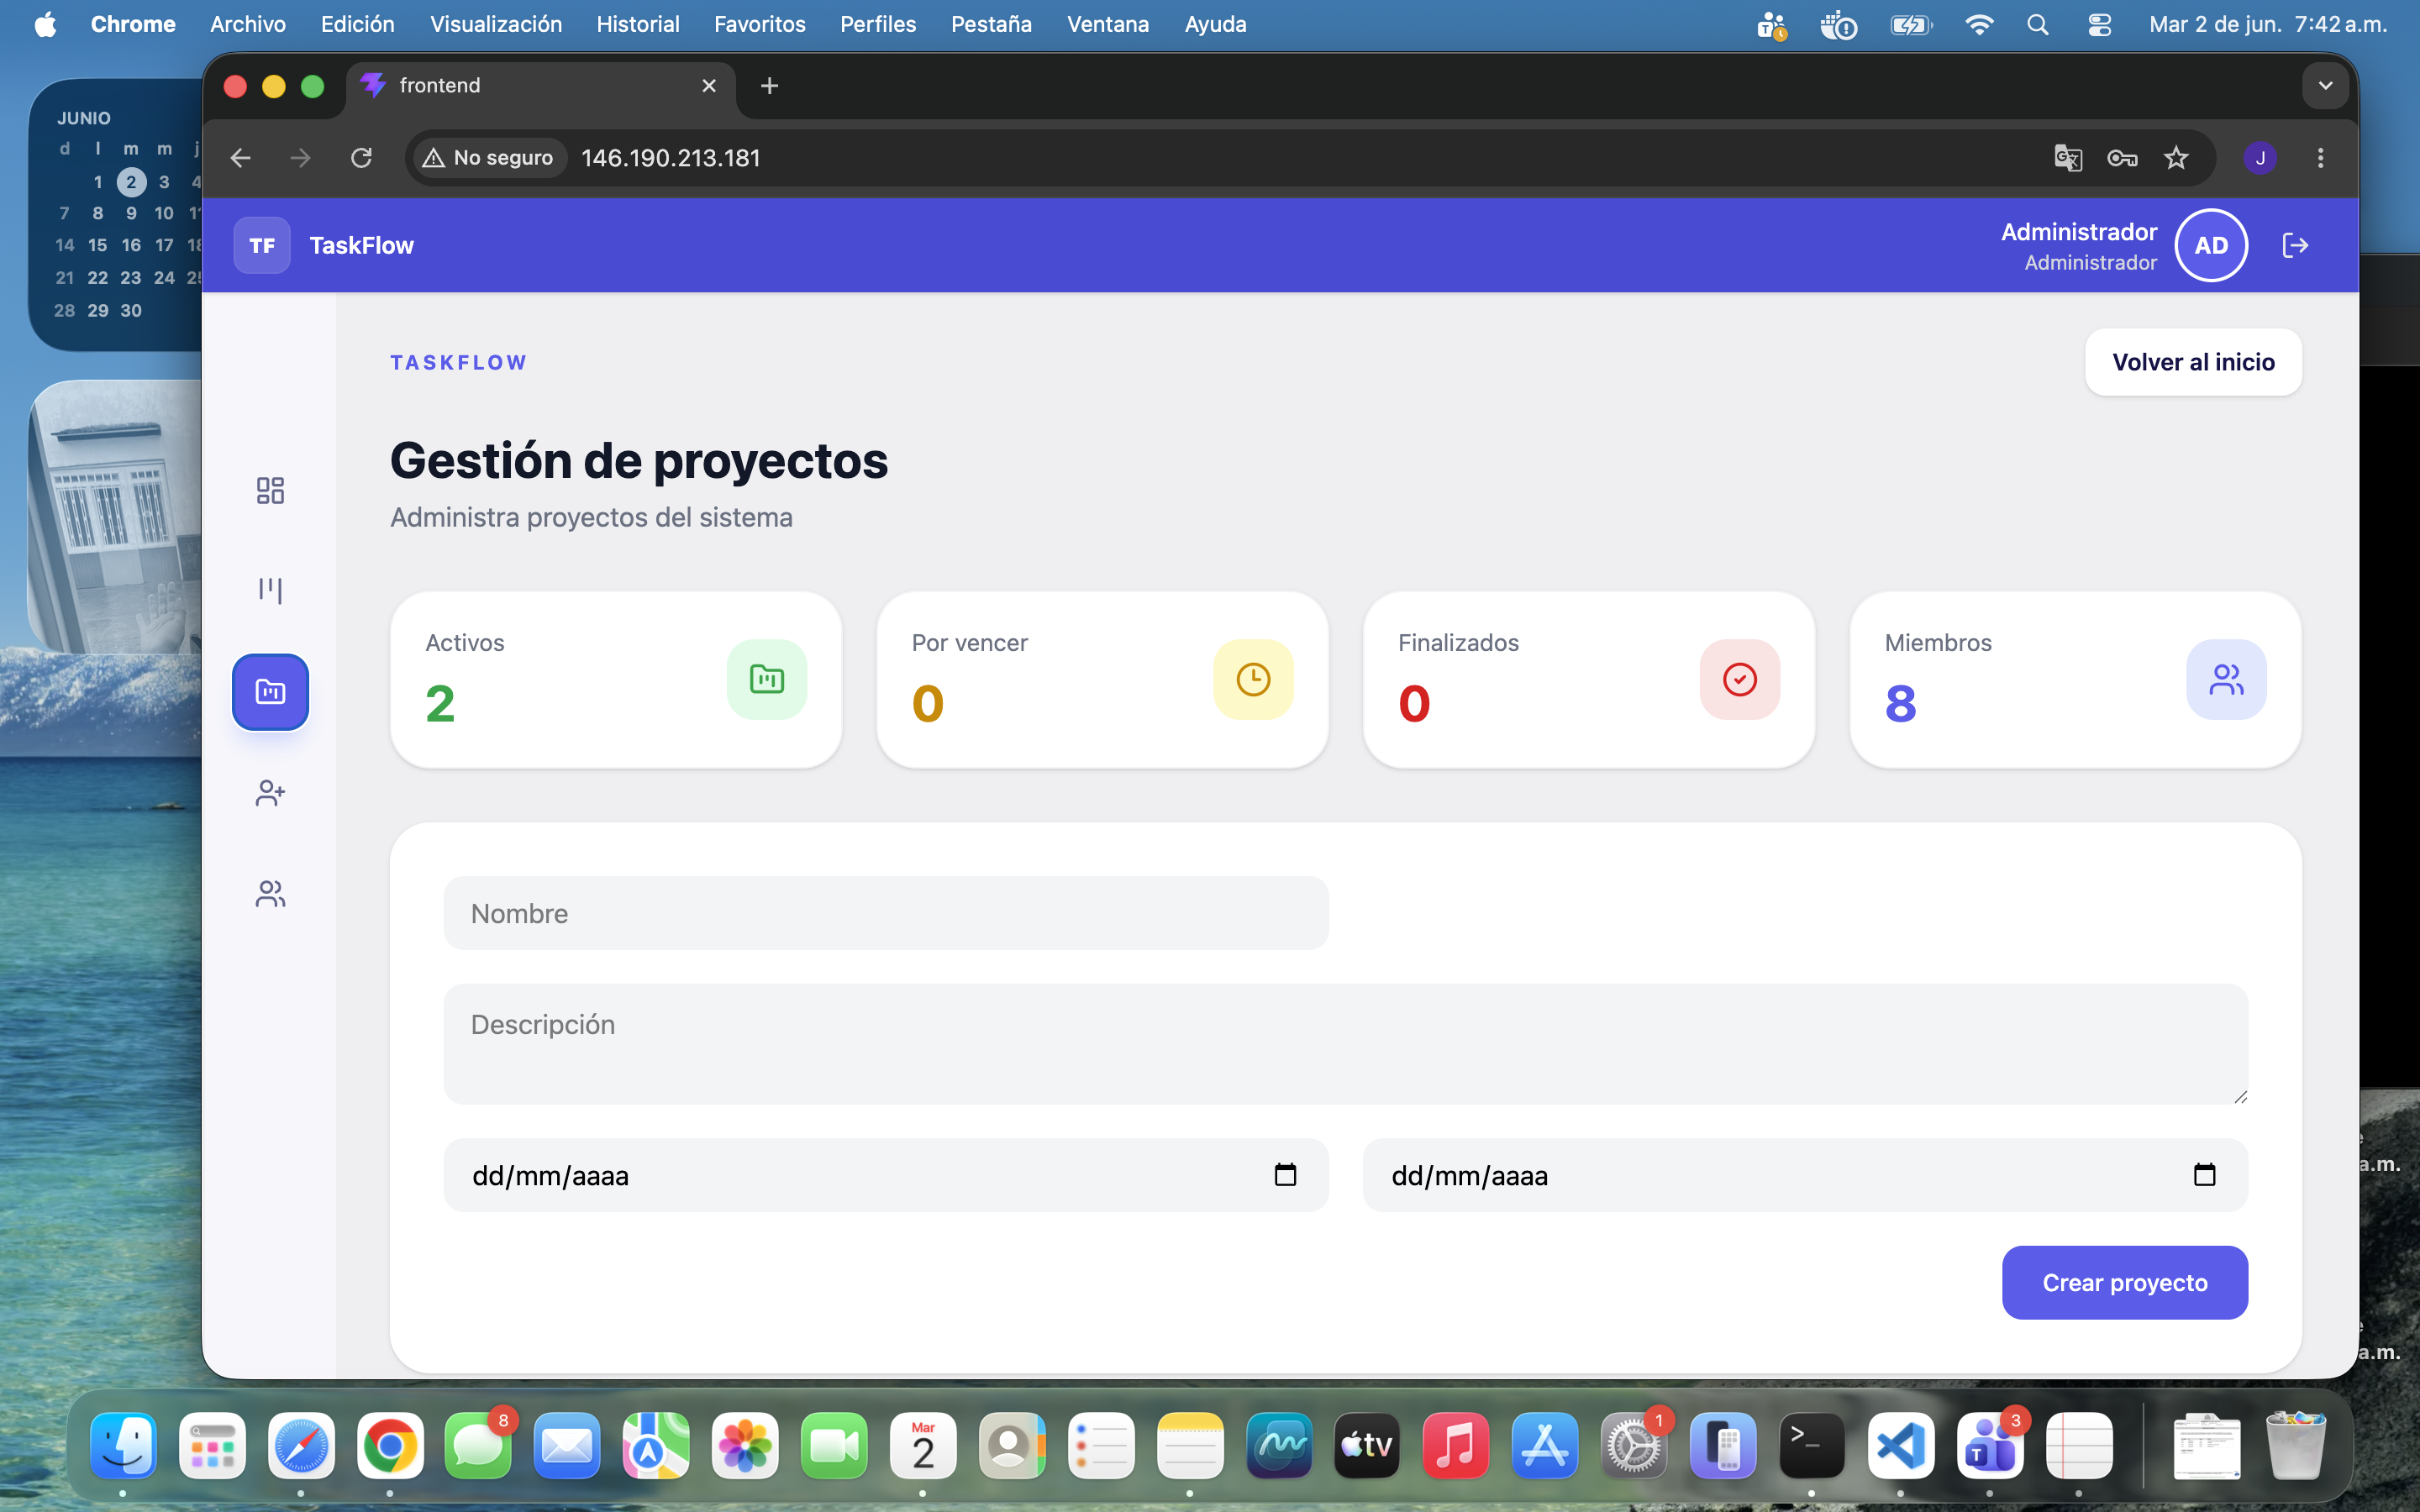
\includegraphics[width=0.90\textwidth]{gestion-proyectos.png}
  \caption{Módulo de gestión de proyectos}
\end{figure}

\subsection{Crear un proyecto}

\textbf{Pasos:}
\begin{enumerate}
  \item Acceda al módulo \textbf{Proyectos} desde la barra de navegación.
  \item Presione el botón \textbf{«+ Nuevo Proyecto»}.
  \item Complete el formulario con la información requerida.
  \item Presione \textbf{«Guardar»} para confirmar la creación.
\end{enumerate}

\textbf{Campos del formulario:}

\begin{table}[H]
\centering
\begin{tabularx}{\textwidth}{L{3.5cm} C{2.2cm} L{7.5cm}}
\toprule
\textbf{Campo} & \textbf{Obligatorio} & \textbf{Descripción} \\
\midrule
Nombre        & Sí  & Identificador único del proyecto. \\
Descripción   & No  & Propósito u objetivo general del proyecto. \\
Fecha de inicio & No & Fecha planificada de inicio del trabajo. \\
Fecha límite  & No  & Fecha estimada de entrega o cierre. \\
\bottomrule
\end{tabularx}
\caption{Campos para la creación de proyectos}
\end{table}

\begin{infobox}[Fases automáticas]
Al crear un proyecto, el sistema genera automáticamente tres fases por defecto: \textbf{Por hacer}, \textbf{En proceso} y \textbf{Finalizado}. Estas fases pueden ser renombradas o eliminadas, y es posible agregar fases adicionales.
\end{infobox}

\subsection{Editar un proyecto}

\begin{enumerate}
  \item Localice el proyecto en la lista.
  \item Presione el ícono de edición (\emph{lápiz}).
  \item Modifique los campos deseados.
  \item Presione \textbf{«Guardar»} para confirmar los cambios.
\end{enumerate}

\begin{warningbox}[Validación de fechas]
La fecha límite no puede ser anterior a la fecha de inicio. El sistema mostrará un error de validación si se intenta guardar un rango de fechas inválido.
\end{warningbox}

\subsection{Eliminar un proyecto}

\begin{enumerate}
  \item Presione el ícono de eliminación (\emph{papelera}) junto al proyecto.
  \item Confirme la acción en el diálogo de confirmación.
\end{enumerate}

\begin{warningbox}[Acción irreversible]
Eliminar un proyecto borra en cascada todas sus fases, tareas, comentarios y registros de tiempo asociados. Esta acción no puede deshacerse.
\end{warningbox}

\subsection{Gestión de fases personalizadas}

Cada proyecto puede tener fases adicionales a las tres predeterminadas.

\subsubsection{Agregar una fase}

\begin{enumerate}
  \item Dentro del proyecto, acceda a la configuración de fases.
  \item Presione \textbf{«+ Agregar Fase»}.
  \item Indique el nombre de la nueva fase.
  \item Confirme para crearla. La fase aparecerá como una nueva columna en el Kanban.
\end{enumerate}

\subsubsection{Renombrar o eliminar una fase}

\begin{itemize}
  \item \textbf{Renombrar:} Seleccione la fase y edite su nombre directamente.
  \item \textbf{Eliminar:} Presione el ícono correspondiente. Las tareas en esa fase serán eliminadas en cascada.
\end{itemize}

% ═══════════════════════════════════════════════════════════════════════════════
\section{Tablero Kanban}

\begin{notebox}
\textbf{Roles con acceso:} \admin\ \leader\ \executor
\end{notebox}

\subsection{Descripción}

El tablero Kanban es la vista central de gestión del trabajo. Muestra las tareas organizadas por fases en columnas, permitiendo visualizar el avance del proyecto de un vistazo.

\begin{figure}[H]
  \centering
  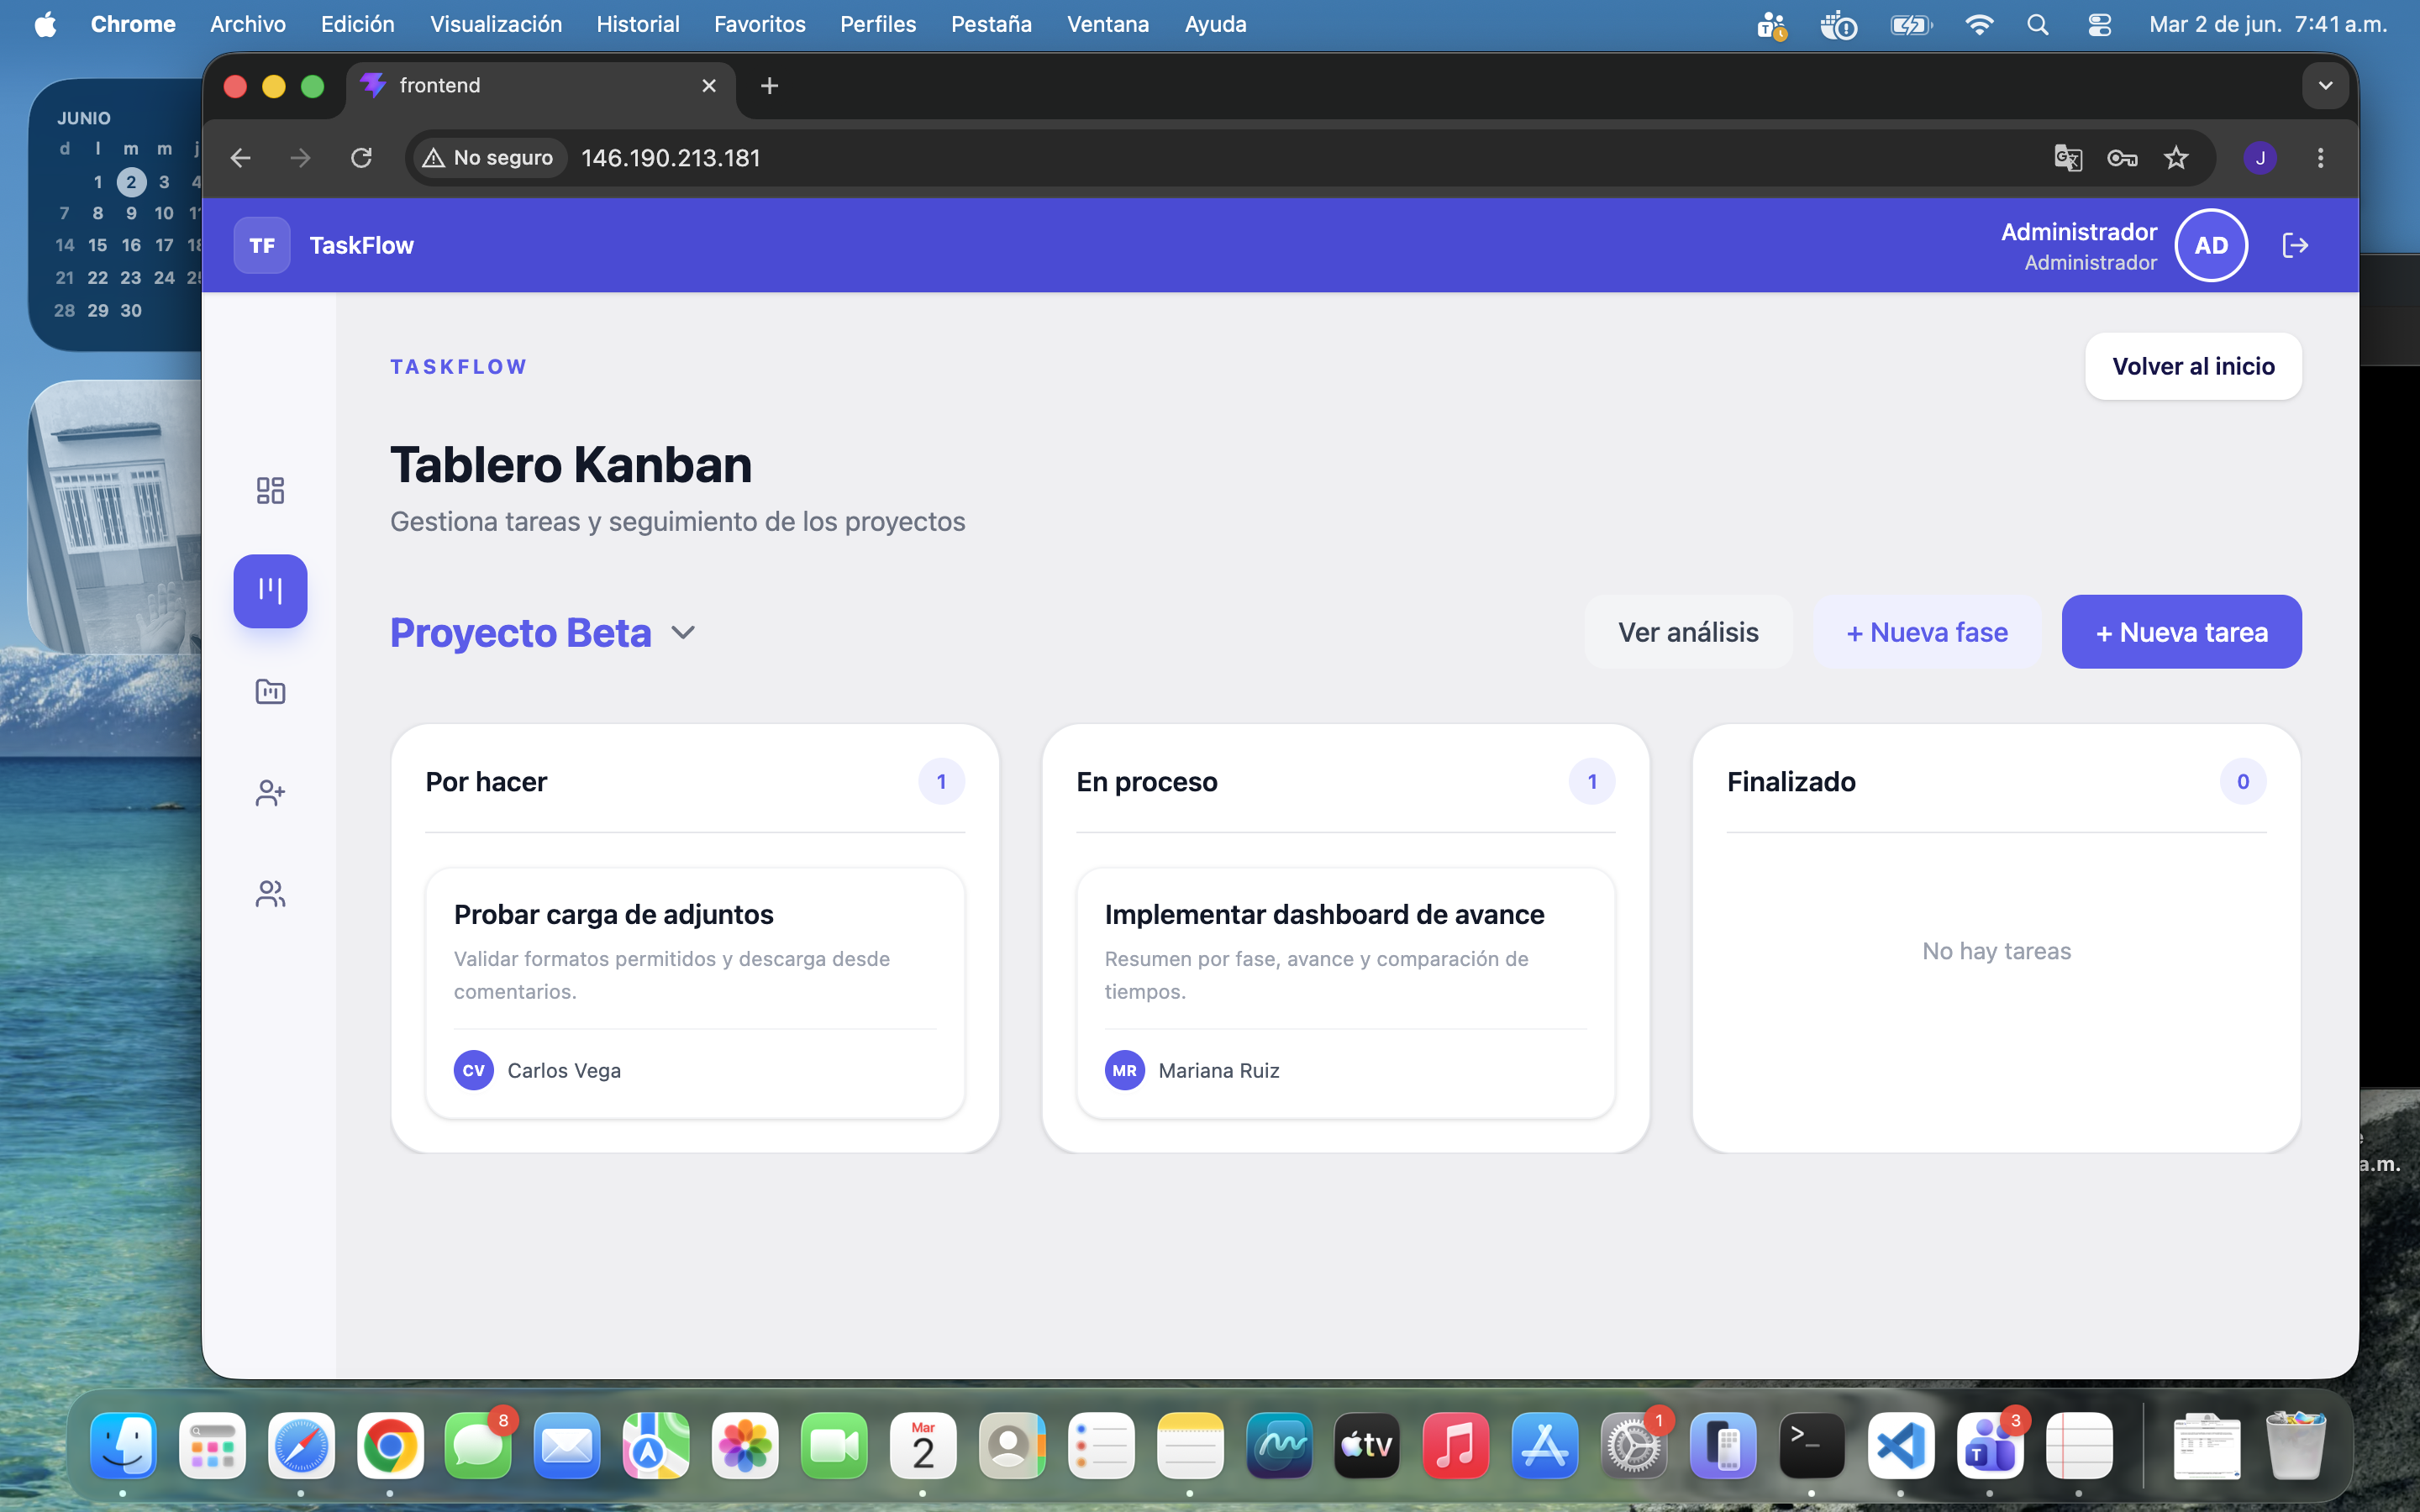
\includegraphics[width=0.95\textwidth]{tablero-kanban.png}
  \caption{Tablero Kanban con fases y tarjetas de tareas}
\end{figure}

\subsection{Estructura del tablero}

Cada columna del tablero representa una \textbf{fase del proyecto}. Las columnas predeterminadas son:

\begin{table}[H]
\centering
\begin{tabularx}{\textwidth}{C{2.5cm} L{6cm} L{5cm}}
\toprule
\textbf{Fase} & \textbf{Significado} & \textbf{Tareas típicas} \\
\midrule
Por hacer    & Tareas planificadas aún no iniciadas & Backlog, tareas nuevas \\
En proceso   & Tareas actualmente en ejecución      & Desarrollo, redacción \\
Finalizado   & Tareas completadas                   & Entregables aprobados \\
Personalizadas & Fases adicionales del proyecto     & Revisión, QA, etc. \\
\bottomrule
\end{tabularx}
\caption{Fases del tablero Kanban}
\end{table}

\subsection{Interacciones con el tablero}

\subsubsection{Mover una tarea entre fases}

\begin{itemize}
  \item \textbf{ADMIN / LÍDER:} Pueden mover cualquier tarea a cualquier fase.
  \item \textbf{EJECUTOR:} Puede mover únicamente las tareas que le estén asignadas.
\end{itemize}

Para mover una tarea, utilice el selector de fase en el detalle de la tarea o arrastre la tarjeta hasta la columna deseada.

\subsubsection{Crear una tarea desde el tablero}

\begin{enumerate}
  \item Presione el botón \textbf{«+ Agregar tarea»} en la columna deseada.
  \item Complete el formulario de creación de tarea (ver sección \ref{sec:tareas}).
  \item La tarea aparecerá directamente en la fase correspondiente.
\end{enumerate}

\subsubsection{Ver el detalle de una tarea}

Haga clic sobre la tarjeta de la tarea para abrir el panel de detalle, donde podrá visualizar toda la información, comentarios y registros de tiempo.

\subsubsection{Resumen del proyecto}

Dentro del tablero existe un botón para mostrar u ocultar el \textbf{dashboard de resumen del proyecto}, que presenta métricas de avance en tiempo real.

% ═══════════════════════════════════════════════════════════════════════════════
\section{Gestión de Tareas}
\label{sec:tareas}

\begin{notebox}
\textbf{Crear / Editar / Eliminar:} \admin\ \leader \quad
\textbf{Mover / Registrar tiempo / Comentar:} \admin\ \leader\ \executor
\end{notebox}

\subsection{Información de una tarea}

Cada tarea puede contener los siguientes campos:

\begin{table}[H]
\centering
\begin{tabularx}{\textwidth}{L{3.8cm} C{2.2cm} L{7.5cm}}
\toprule
\textbf{Campo} & \textbf{Obligatorio} & \textbf{Descripción} \\
\midrule
Título          & Sí  & Nombre descriptivo de la tarea. \\
Descripción     & No  & Detalle de lo que debe realizarse. \\
Fase            & Sí  & Columna del Kanban donde se ubica la tarea. \\
Responsable     & No  & Usuario asignado (debe ser miembro del proyecto). \\
Fecha de inicio & No  & Fecha planificada de comienzo de la tarea. \\
Fecha límite    & No  & Plazo de entrega de la tarea. \\
Tiempo estimado & No  & Horas previstas para completar la tarea. \\
\bottomrule
\end{tabularx}
\caption{Campos disponibles en una tarea}
\end{table}

\begin{figure}[H]
  \centering
  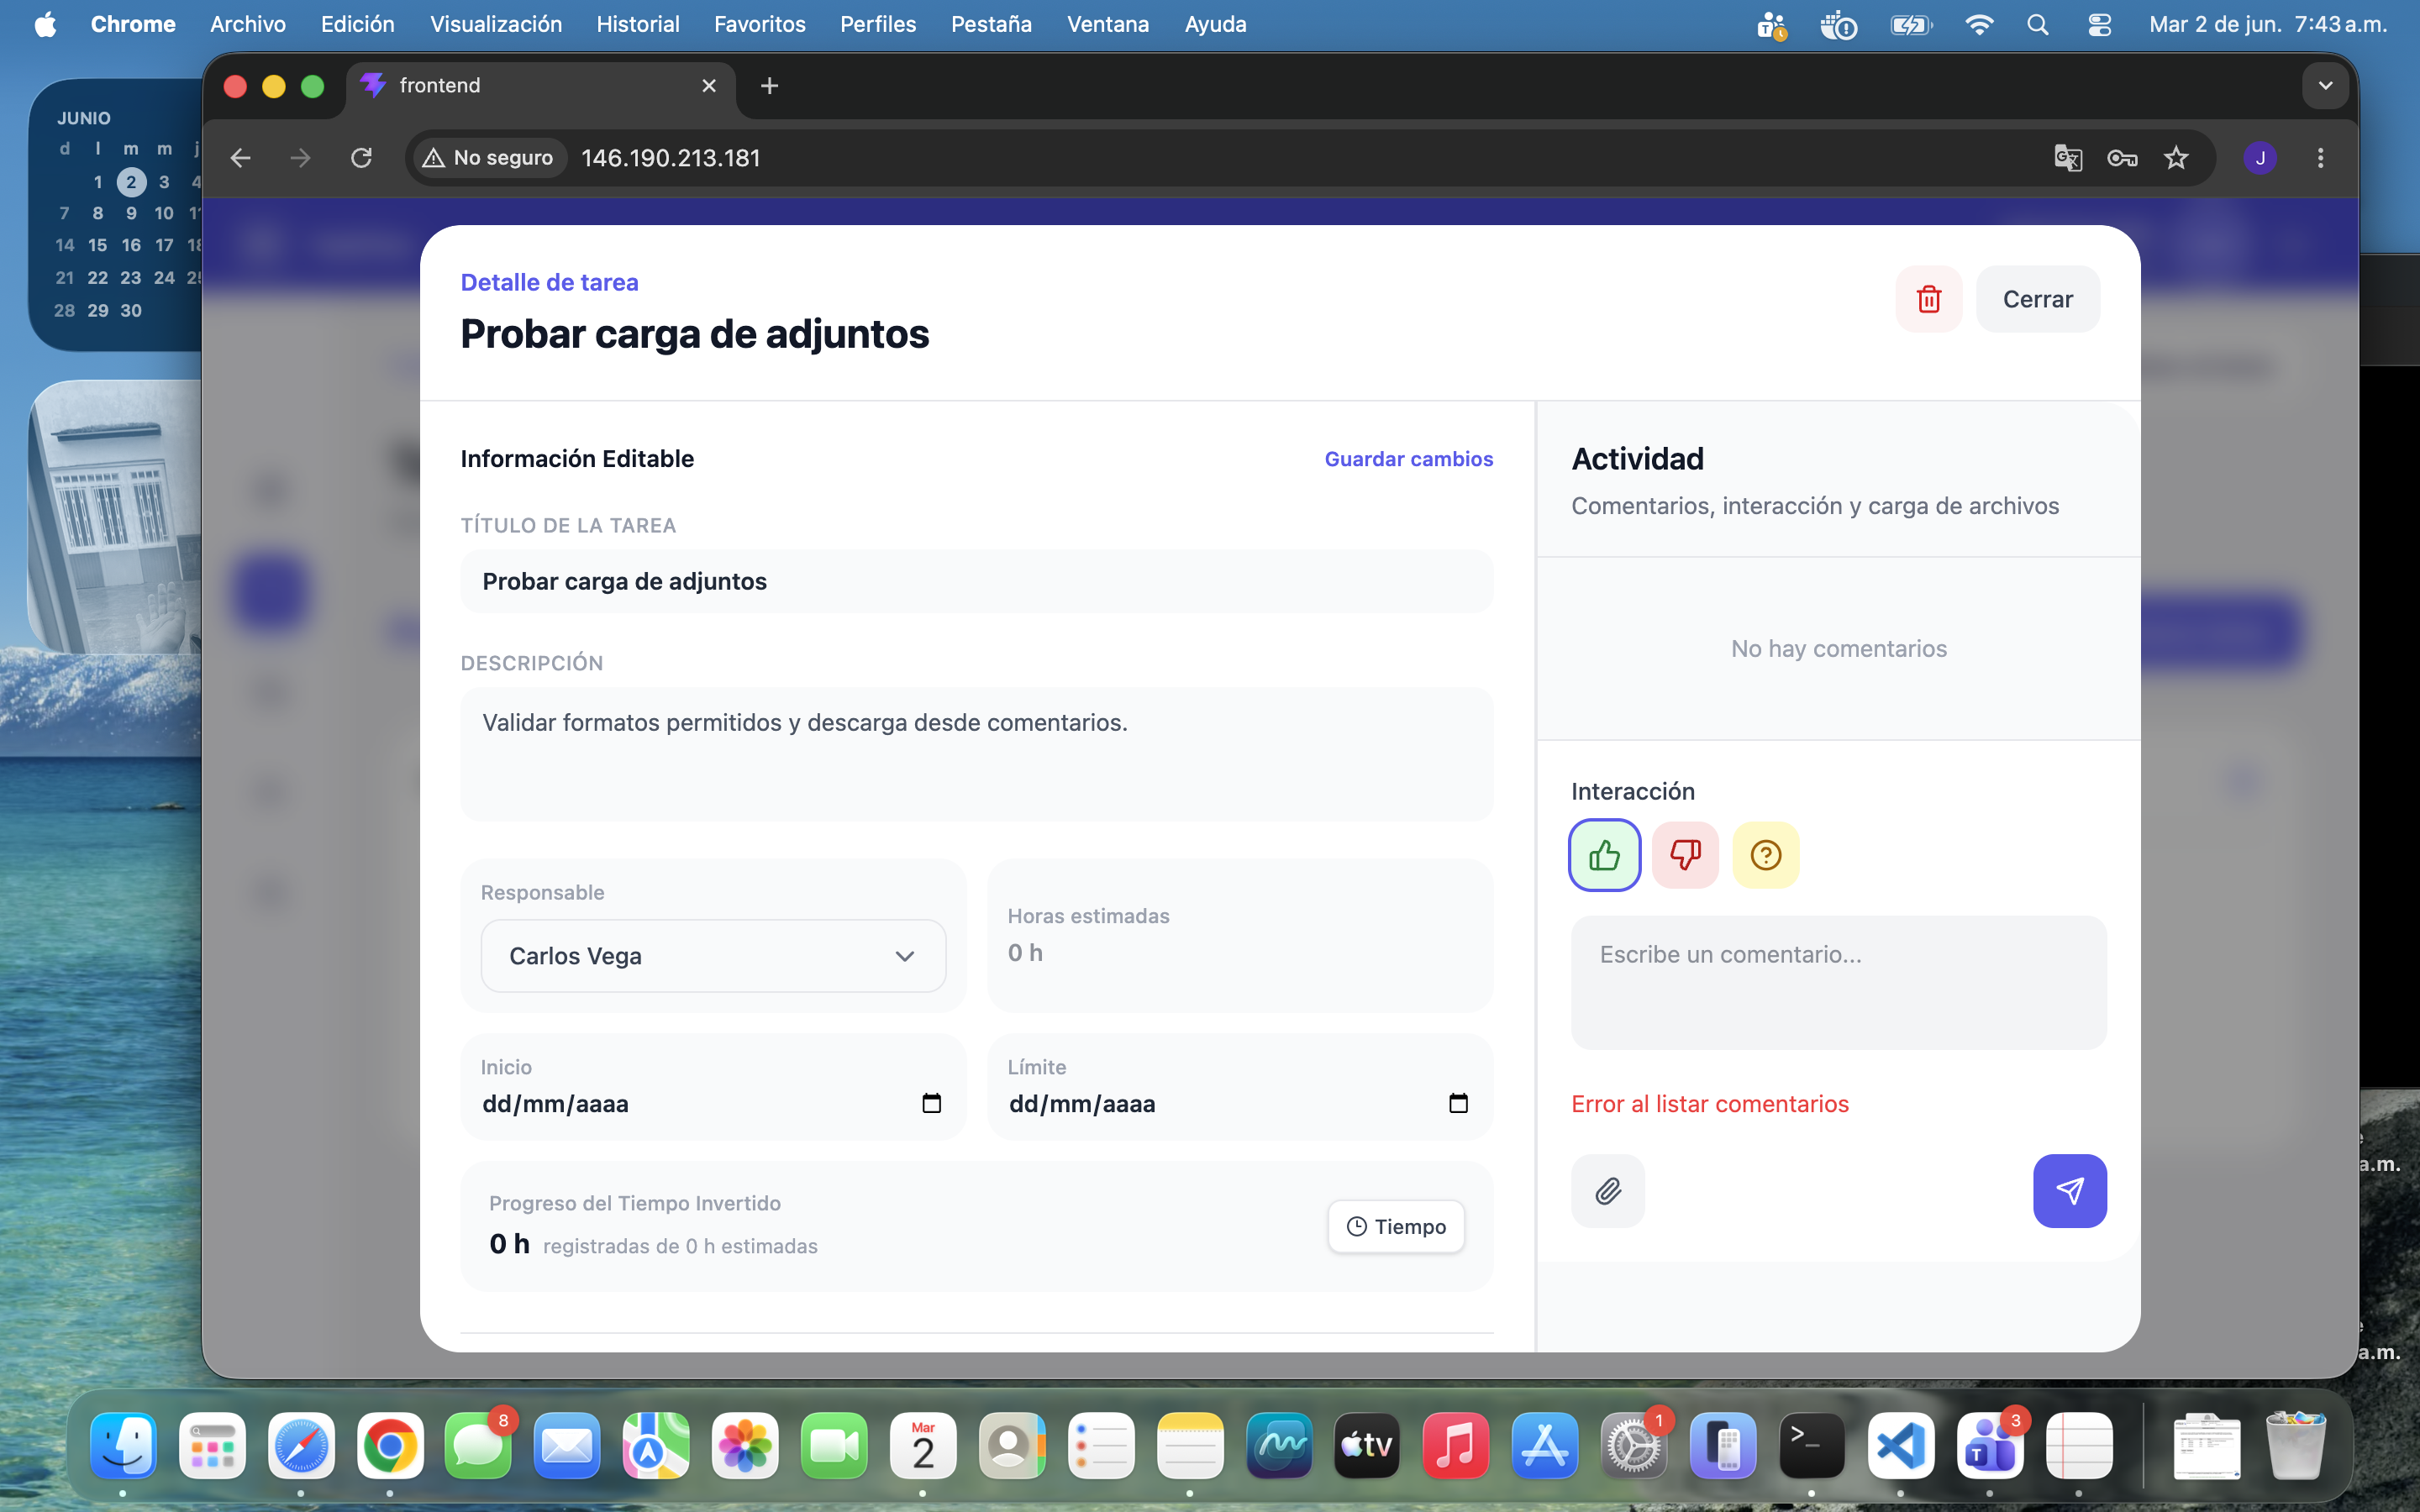
\includegraphics[width=0.88\textwidth]{editar-tarea-comentarios.png}
  \caption{Formulario de edición de tarea con panel de comentarios}
\end{figure}

\subsection{Crear una tarea}

\begin{enumerate}
  \item Desde el tablero Kanban, presione \textbf{«+ Agregar tarea»} en la fase deseada, o use el botón de nueva tarea en la vista de listado.
  \item Complete los campos del formulario.
  \item Asigne un responsable si corresponde (solo usuarios miembros del proyecto).
  \item Presione \textbf{«Guardar»}.
\end{enumerate}

\begin{infobox}[Validación de responsable]
Solo pueden asignarse como responsable usuarios que ya sean miembros del proyecto. Si se intenta asignar a otro usuario, el sistema rechazará la operación.
\end{infobox}

\subsection{Editar una tarea}

\begin{enumerate}
  \item Haga clic sobre la tarea en el tablero Kanban para abrirla.
  \item Modifique los campos necesarios en el panel de edición.
  \item Los cambios se guardan automáticamente o mediante el botón \textbf{«Actualizar»}.
\end{enumerate}

\subsection{Eliminar una tarea}

\begin{enumerate}
  \item Abra la tarea desde el tablero.
  \item Presione el botón \textbf{«Eliminar»}.
  \item Confirme la acción en el diálogo de confirmación.
\end{enumerate}

\begin{warningbox}[Acción irreversible]
Al eliminar una tarea se borran también todos sus comentarios, archivos adjuntos y registros de tiempo.
\end{warningbox}

\subsection{Indicadores de alerta en tareas}

El sistema calcula automáticamente si una tarea está \textbf{vencida}: cuando la fecha límite es anterior a la fecha actual y la tarea no se encuentra en la fase «Finalizado». Las tarjetas vencidas se muestran con una indicación visual de alerta.

\subsection{Registro de tiempo}
\label{sec:tiempo}

\begin{notebox}
\textbf{Roles con acceso:} Solo el \executor\ o usuario asignado a la tarea.
\end{notebox}

El registro de tiempo permite documentar el esfuerzo real invertido en una tarea.

\textbf{Pasos:}
\begin{enumerate}
  \item Abra la tarea asignada a usted.
  \item Localice la sección \textbf{«Registrar Tiempo»}.
  \item Ingrese la cantidad de minutos trabajados.
  \item (Opcional) Añada una descripción de lo realizado.
  \item Presione \textbf{«Registrar»}.
\end{enumerate}

\textbf{Datos registrados por entrada:}
\begin{itemize}
  \item Usuario que registra el tiempo.
  \item Minutos trabajados.
  \item Descripción (opcional).
  \item Fecha y hora del registro.
\end{itemize}

Los registros de tiempo se acumulan y son utilizados en el dashboard de resumen para comparar \textbf{horas estimadas vs. horas reales}.

% ═══════════════════════════════════════════════════════════════════════════════
\section{Comentarios y Seguimiento}

\begin{notebox}
\textbf{Roles con acceso:} Cualquier usuario con acceso a la tarea (\admin, \leader\ o miembro del proyecto con tarea asignada).
\end{notebox}

\subsection{Panel de actividad}

Cada tarea dispone de un panel de actividad donde se registran los comentarios del equipo. Este panel constituye el historial de seguimiento de la tarea.

\subsection{Crear un comentario}

\begin{enumerate}
  \item Abra la tarea desde el tablero Kanban.
  \item En la sección \textbf{«Comentarios»}, escriba el contenido del comentario.
  \item Seleccione el \textbf{tipo de interacción}:
  \begin{itemize}
    \item \textcolor{success}{\textbf{Aprobado}} — El trabajo revisado es correcto o se acepta.
    \item \textcolor{danger}{\textbf{Desaprobado}} — El trabajo tiene observaciones y debe corregirse.
    \item \textcolor{warning}{\textbf{Duda}} — Se plantea una pregunta sobre la tarea.
  \end{itemize}
  \item (Opcional) Adjunte archivos usando el botón de adjuntos.
  \item Presione \textbf{«Publicar»}.
\end{enumerate}

\subsection{Archivos adjuntos}

Es posible adjuntar archivos a un comentario para compartir evidencias, documentos o capturas de pantalla.

\textbf{Especificaciones:}

\begin{table}[H]
\centering
\begin{tabularx}{\textwidth}{L{3.5cm} L{9.5cm}}
\toprule
\textbf{Parámetro} & \textbf{Valor} \\
\midrule
Formatos permitidos & PDF, DOCX, DOC, TXT, XLSX, XLS, PNG, JPG, JPEG \\
Tamaño máximo       & 10 MB por archivo \\
Cantidad            & Múltiples archivos por comentario \\
\bottomrule
\end{tabularx}
\caption{Especificaciones para archivos adjuntos}
\end{table}

\begin{warningbox}[Formato no permitido]
Si intenta cargar un archivo con una extensión no permitida o que supere el límite de tamaño, el sistema rechazará el archivo y mostrará un mensaje de error.
\end{warningbox}

\subsection{Historial de comentarios}

Los comentarios se muestran en orden cronológico ascendente. Cada comentario incluye:
\begin{itemize}
  \item Nombre del usuario que lo publicó.
  \item Tipo de interacción (ícono de color).
  \item Contenido del comentario.
  \item Archivos adjuntos descargables.
  \item Fecha y hora de publicación.
\end{itemize}

% ═══════════════════════════════════════════════════════════════════════════════
\section{Dashboard de Resumen del Proyecto}

\begin{notebox}
\textbf{Roles con acceso:} \admin\ \leader\ y \executor\ que sean miembros del proyecto.
\end{notebox}

\subsection{Descripción}

El dashboard de resumen proporciona una vista consolidada del estado actual del proyecto con métricas calculadas en tiempo real.

\subsection{Métricas disponibles}

\begin{table}[H]
\centering
\begin{tabularx}{\textwidth}{L{4.5cm} L{9cm}}
\toprule
\textbf{Métrica} & \textbf{Descripción} \\
\midrule
Progreso general &
  Porcentaje de tareas en la fase «Finalizado» respecto al total. \\
\addlinespace
Tareas totales &
  Número total de tareas del proyecto. \\
\addlinespace
Tareas completadas &
  Tareas en fase «Finalizado». \\
\addlinespace
Ejecutores activos &
  Cantidad de ejecutores con al menos una tarea asignada. \\
\addlinespace
Distribución por fase &
  Cantidad y porcentaje de tareas en cada fase del proyecto. \\
\addlinespace
Horas estimadas &
  Suma total de horas estimadas en las tareas del proyecto. \\
\addlinespace
Horas reales &
  Total de horas y minutos registrados mediante registros de tiempo. \\
\bottomrule
\end{tabularx}
\caption{Métricas del dashboard de resumen}
\end{table}

\subsection{Cómo acceder}

Dentro del tablero Kanban, presione el botón \textbf{«Ver resumen del proyecto»}. El panel se desplegará mostrando los indicadores actualizados.

% ═══════════════════════════════════════════════════════════════════════════════
\section{Visualización de Carga Laboral}

\begin{notebox}
\textbf{Roles con acceso:} \admin\ \leader
\end{notebox}

\subsection{Descripción}

El módulo de carga laboral permite monitorear cómo se distribuye el trabajo entre los miembros del equipo, ayudando a detectar desequilibrios y reasignar tareas oportunamente.

\begin{figure}[H]
  \centering
  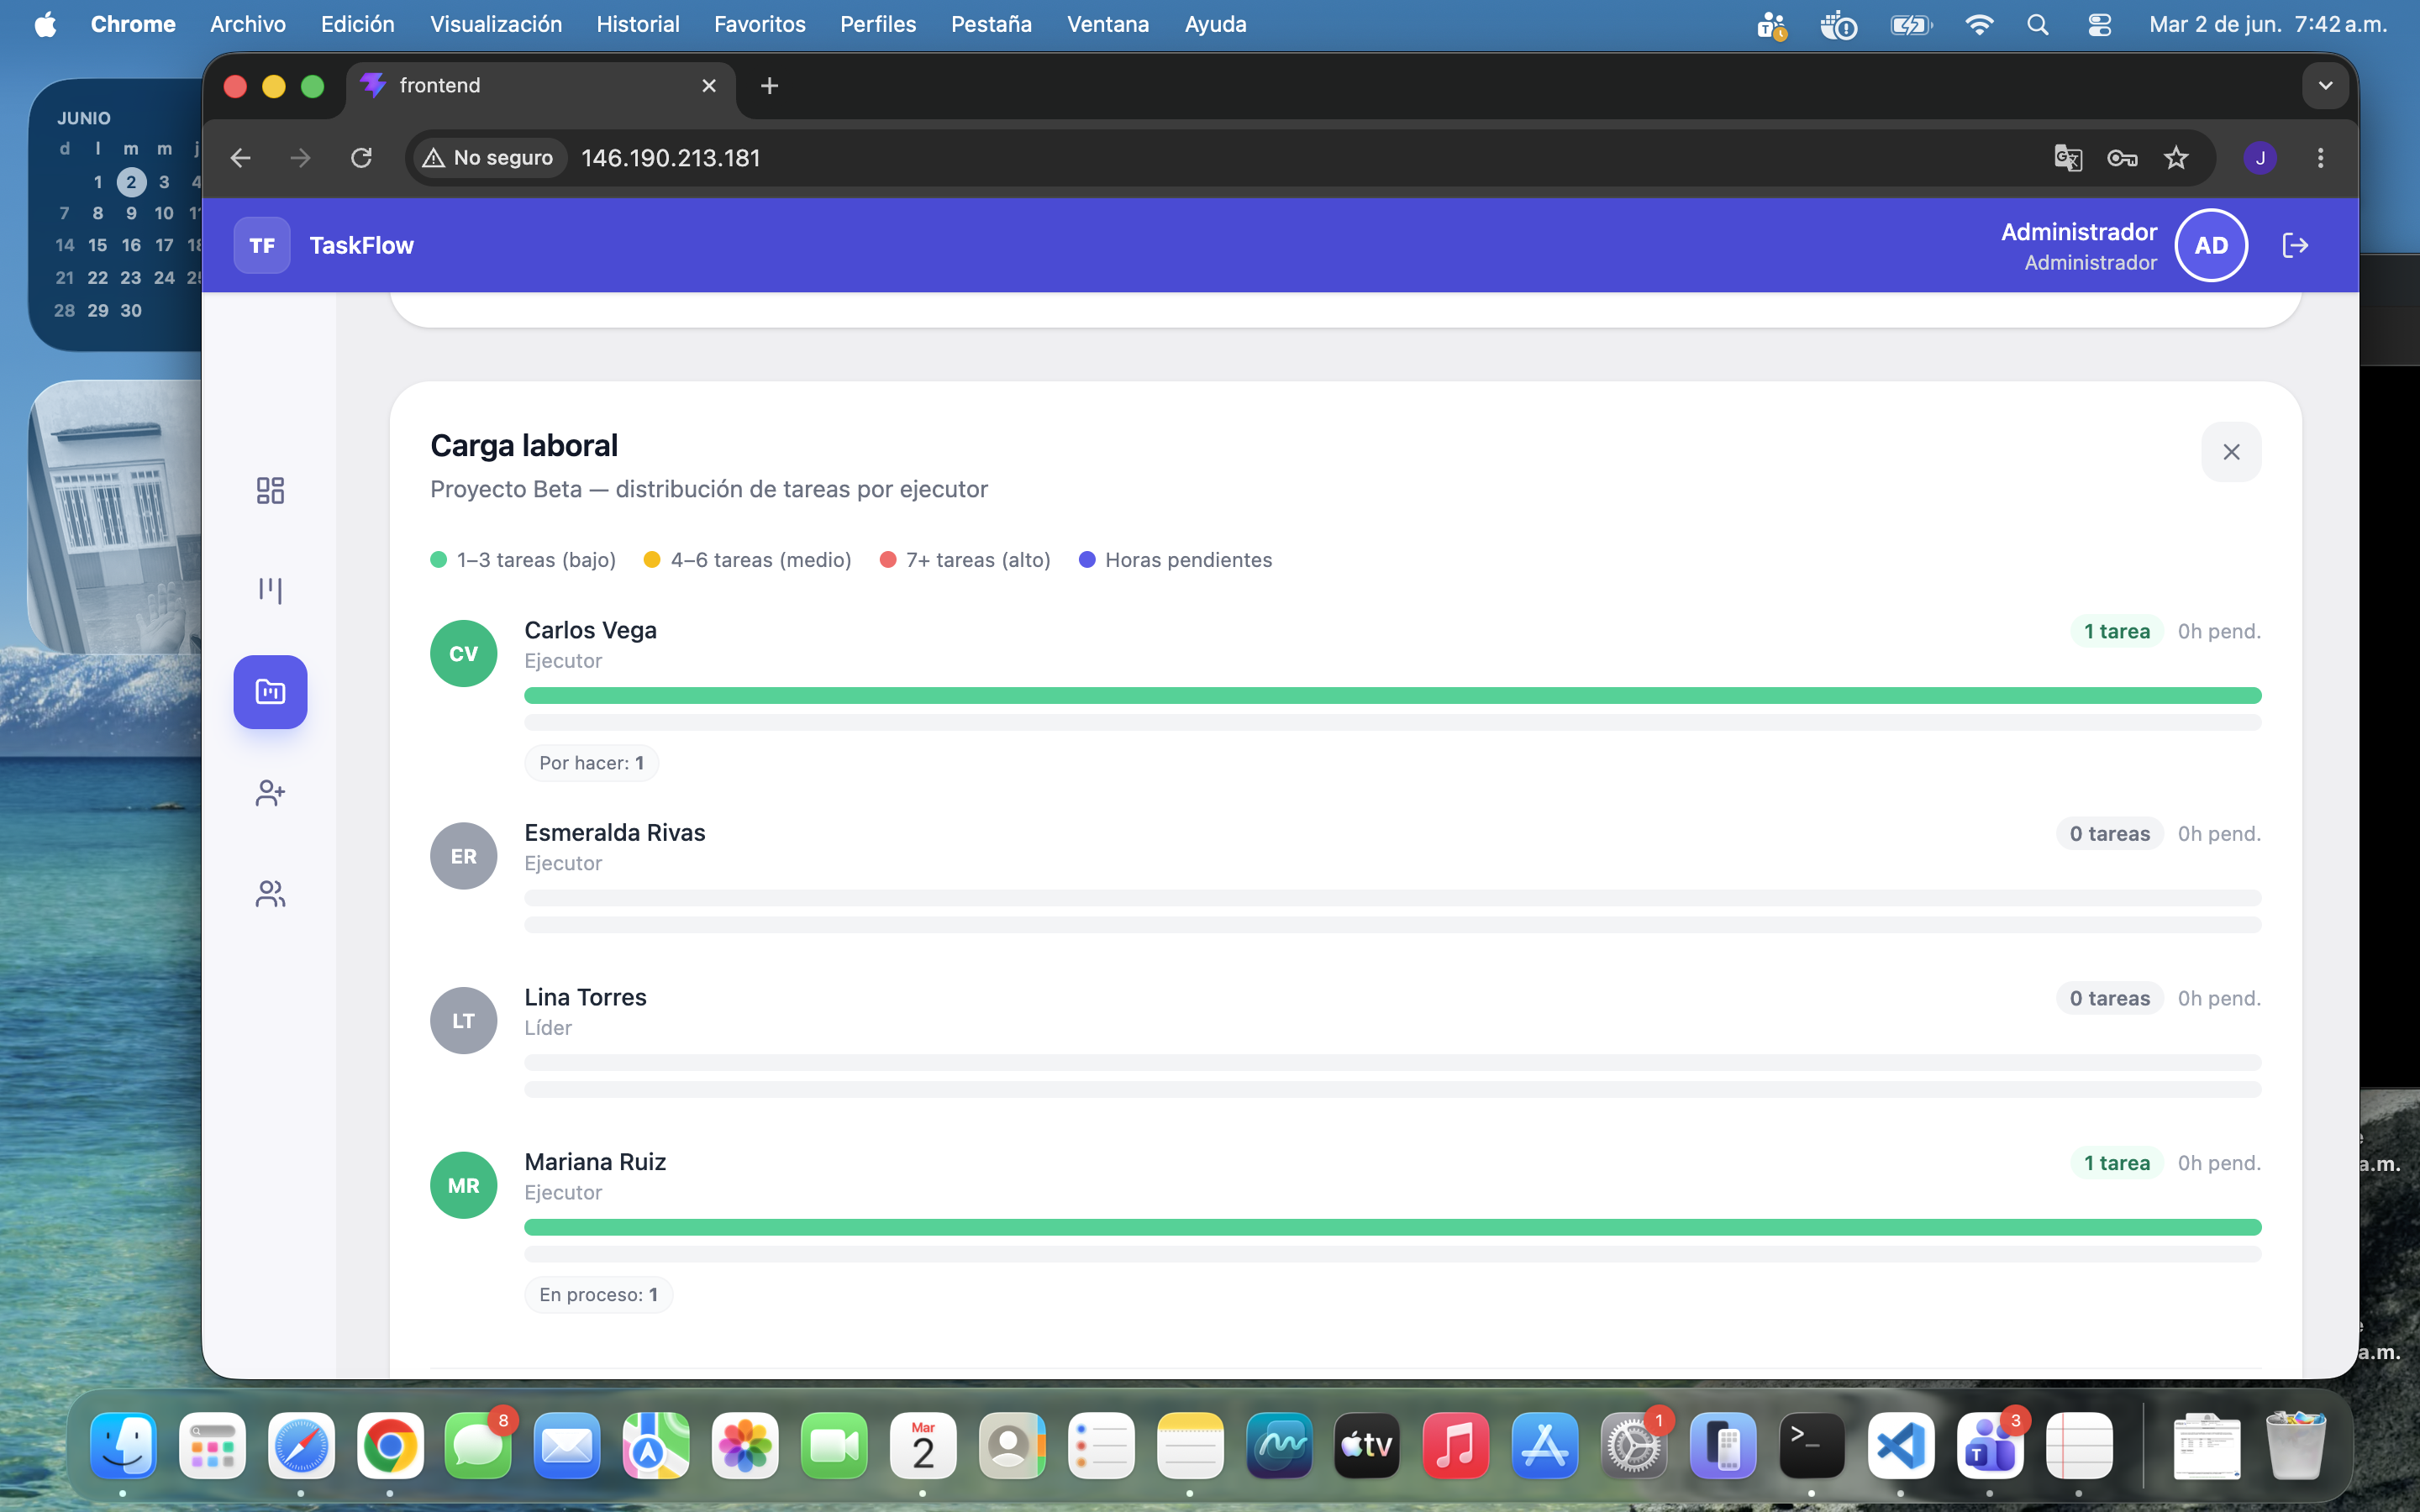
\includegraphics[width=0.90\textwidth]{carga-laboral.png}
  \caption{Vista de distribución de carga laboral}
\end{figure}

\subsection{Información mostrada por usuario}

Para cada miembro del equipo se muestra:

\begin{itemize}
  \item Nombre y correo del usuario.
  \item Total de tareas asignadas.
  \item Horas estimadas pendientes (tareas aún no finalizadas).
  \item Distribución de tareas por estado.
\end{itemize}

\subsection{Código de colores}

El sistema aplica un código de colores para identificar rápidamente el nivel de carga:

\begin{table}[H]
\centering
\begin{tabularx}{\textwidth}{C{2cm} C{3.5cm} L{7.5cm}}
\toprule
\textbf{Color} & \textbf{Rango} & \textbf{Interpretación} \\
\midrule
\textcolor{medgray}{\textbf{Gris}}    & 0 tareas  & Sin carga asignada \\
\textcolor{success}{\textbf{Verde}}   & 1–3 tareas & Carga baja \\
\textcolor{warning}{\textbf{Ámbar}}   & 4–6 tareas & Carga media \\
\textcolor{danger}{\textbf{Rojo}}     & 7+ tareas  & Sobrecarga \\
\bottomrule
\end{tabularx}
\caption{Código de colores de carga laboral}
\end{table}

\begin{infobox}[Recomendación]
Revise periódicamente esta vista para identificar miembros con sobrecarga (marcados en rojo) y redistribuir tareas antes de que afecten los plazos del proyecto.
\end{infobox}

% ═══════════════════════════════════════════════════════════════════════════════
\section{Gestión de Usuarios}

\begin{notebox}
\textbf{Roles con acceso:} Solo \admin
\end{notebox}

\subsection{Descripción}

El módulo de gestión de usuarios permite al administrador del sistema crear, actualizar y eliminar cuentas de usuario, así como gestionar sus roles.

\begin{figure}[H]
  \centering
  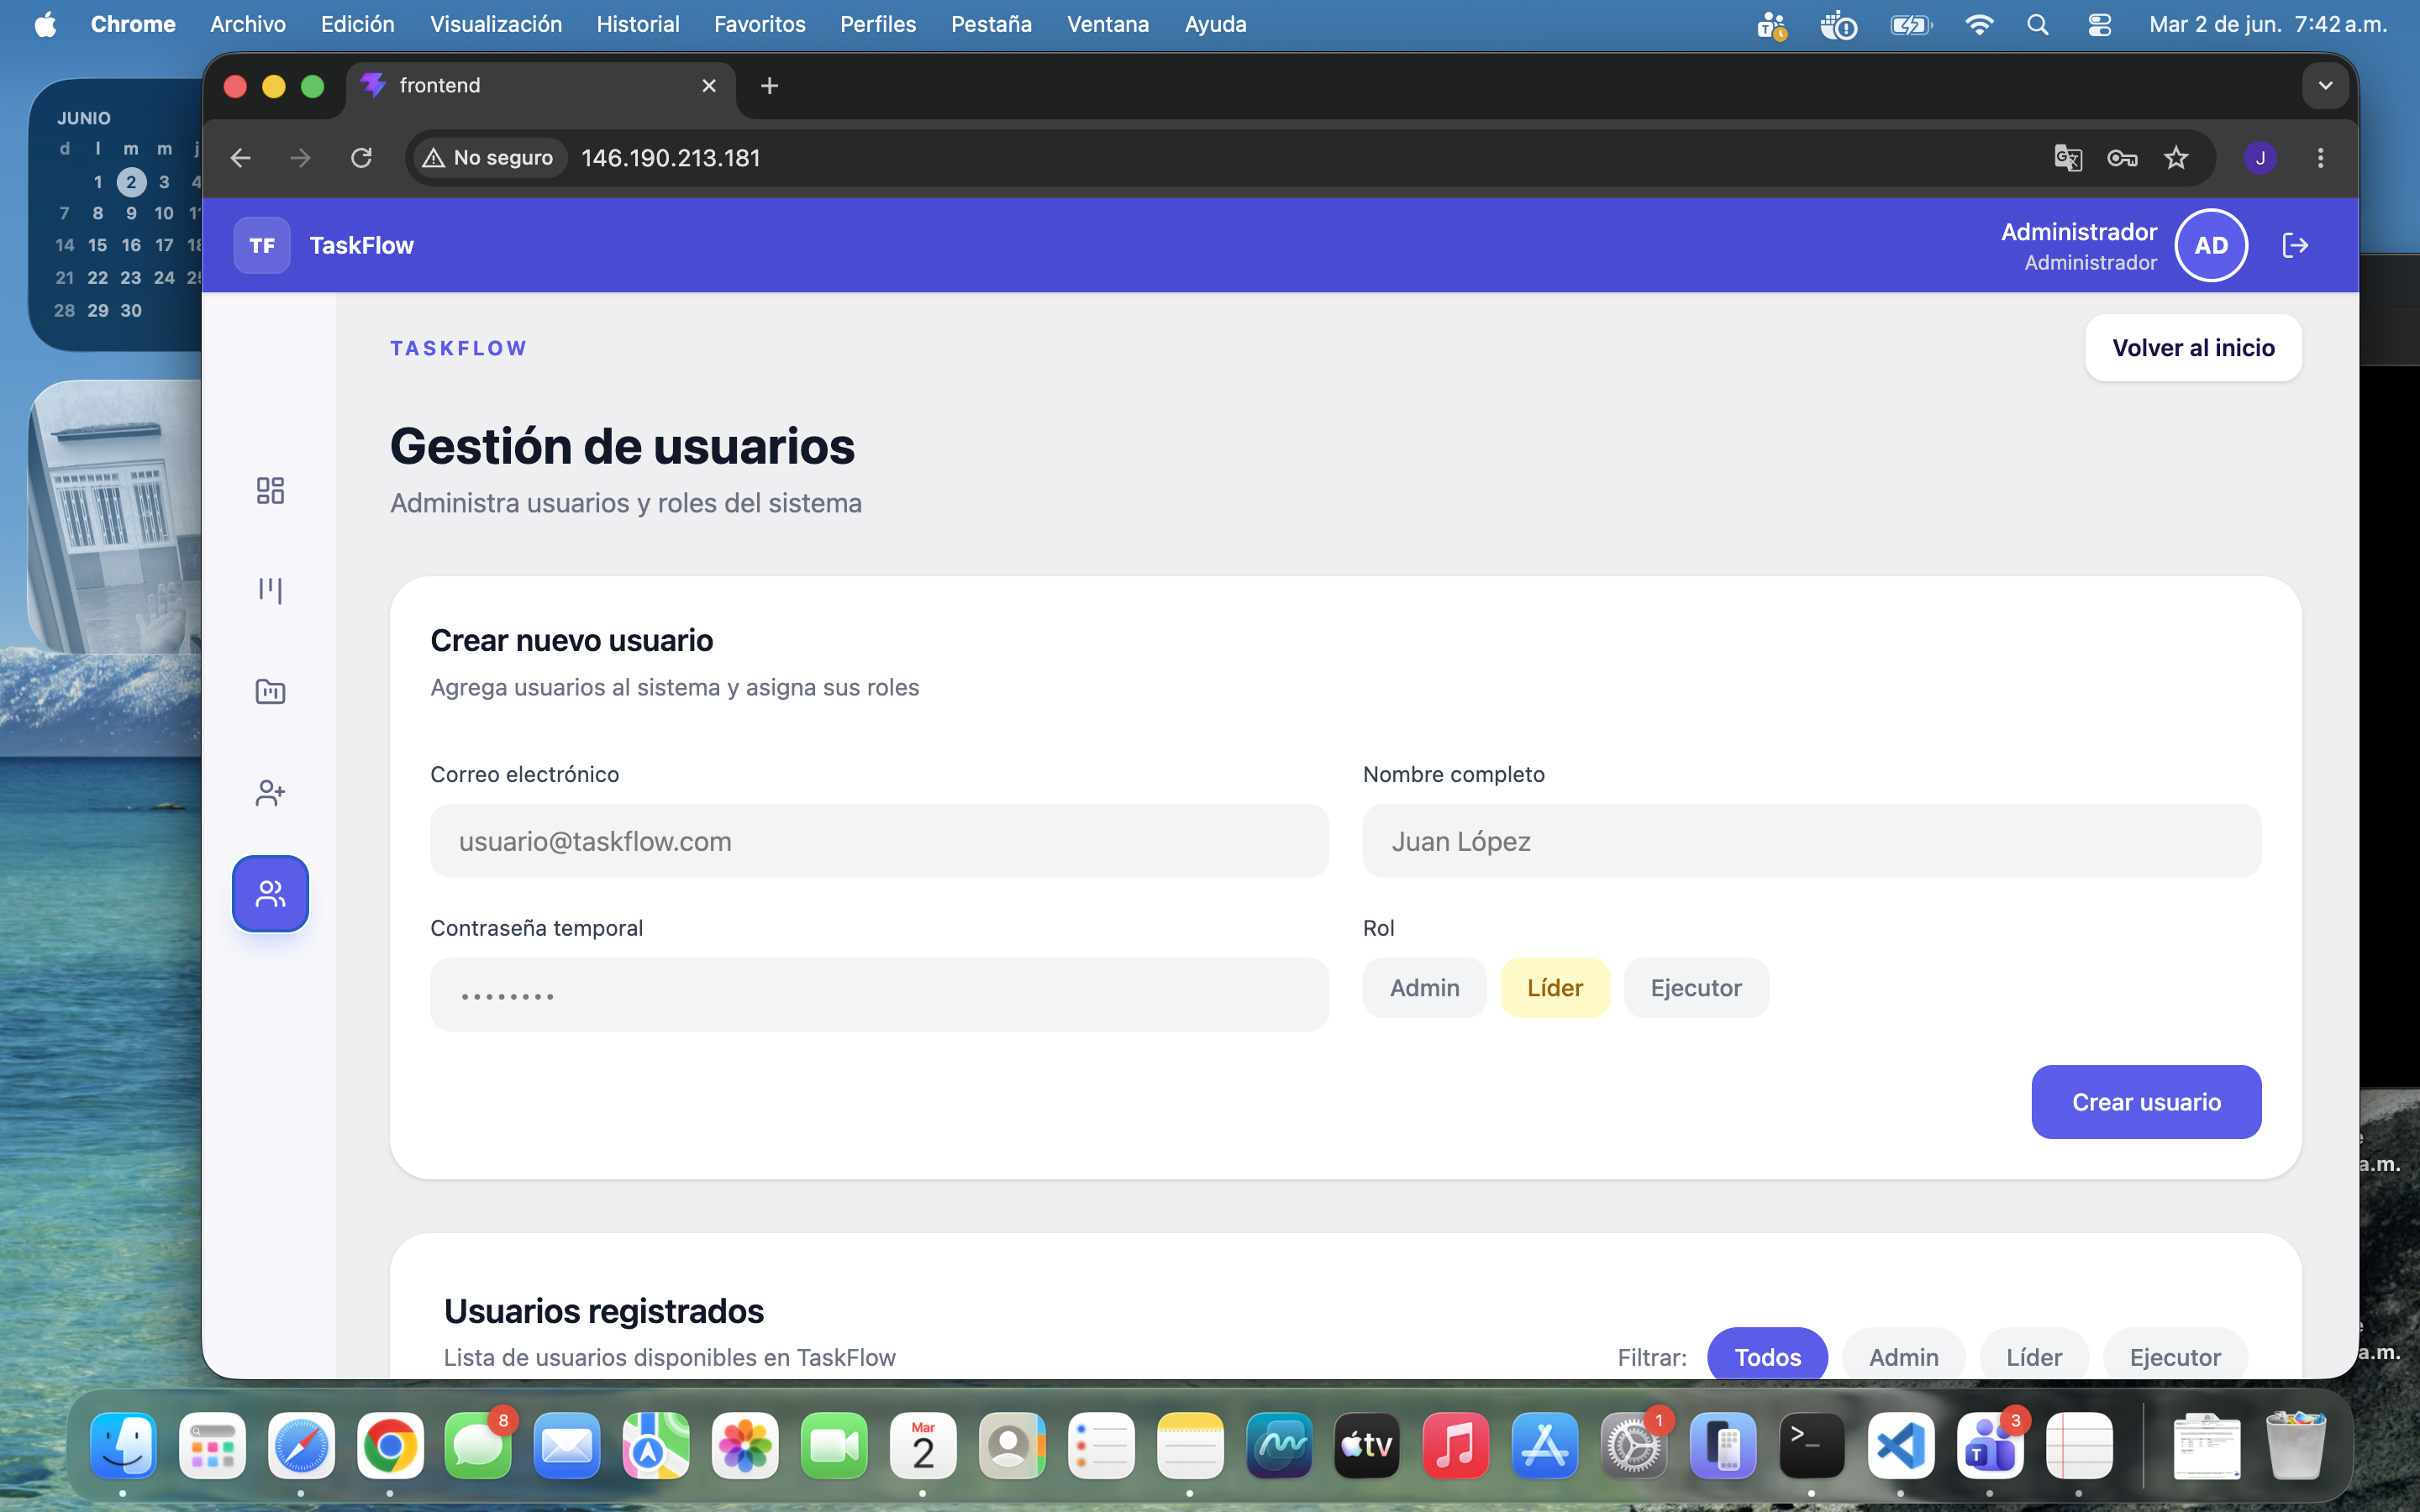
\includegraphics[width=0.90\textwidth]{gestion-usuarios.png}
  \caption{Módulo de gestión de usuarios}
\end{figure}

\subsection{Crear un usuario}

\begin{enumerate}
  \item Acceda al módulo \textbf{Usuarios} desde la barra de navegación.
  \item Presione \textbf{«+ Nuevo Usuario»}.
  \item Complete el formulario con los datos requeridos.
  \item Presione \textbf{«Guardar»}.
\end{enumerate}

\textbf{Campos requeridos:}

\begin{table}[H]
\centering
\begin{tabularx}{\textwidth}{L{3.5cm} C{2.2cm} L{7.5cm}}
\toprule
\textbf{Campo} & \textbf{Obligatorio} & \textbf{Descripción} \\
\midrule
Nombre      & No  & Nombre completo del usuario. \\
Correo      & Sí  & Dirección de correo electrónico única. \\
Contraseña  & Sí  & Contraseña de acceso (se almacena cifrada). \\
Rol         & Sí  & Rol asignado: ADMIN, LÍDER o EJECUTOR. \\
\bottomrule
\end{tabularx}
\caption{Campos para la creación de usuarios}
\end{table}

\subsection{Actualizar un usuario}

\begin{enumerate}
  \item Localice el usuario en la lista.
  \item Presione el ícono de edición.
  \item Modifique el nombre o el rol del usuario.
  \item Presione \textbf{«Guardar»}.
\end{enumerate}

\begin{warningbox}[Restricción de autoedición]
Un administrador no puede cambiar su propio rol desde este módulo, lo que garantiza que siempre exista al menos un administrador activo en el sistema.
\end{warningbox}

\subsection{Eliminar un usuario}

\begin{enumerate}
  \item Localice el usuario en la lista.
  \item Presione el ícono de eliminación.
  \item Confirme la acción.
\end{enumerate}

\begin{warningbox}[Restricciones]
Un administrador no puede eliminarse a sí mismo. Tampoco es posible eliminar usuarios que se encuentren asignados como responsables de tareas activas (se recomienda desasignar primero).
\end{warningbox}

\subsection{Lista de usuarios registrados}

\begin{figure}[H]
  \centering
  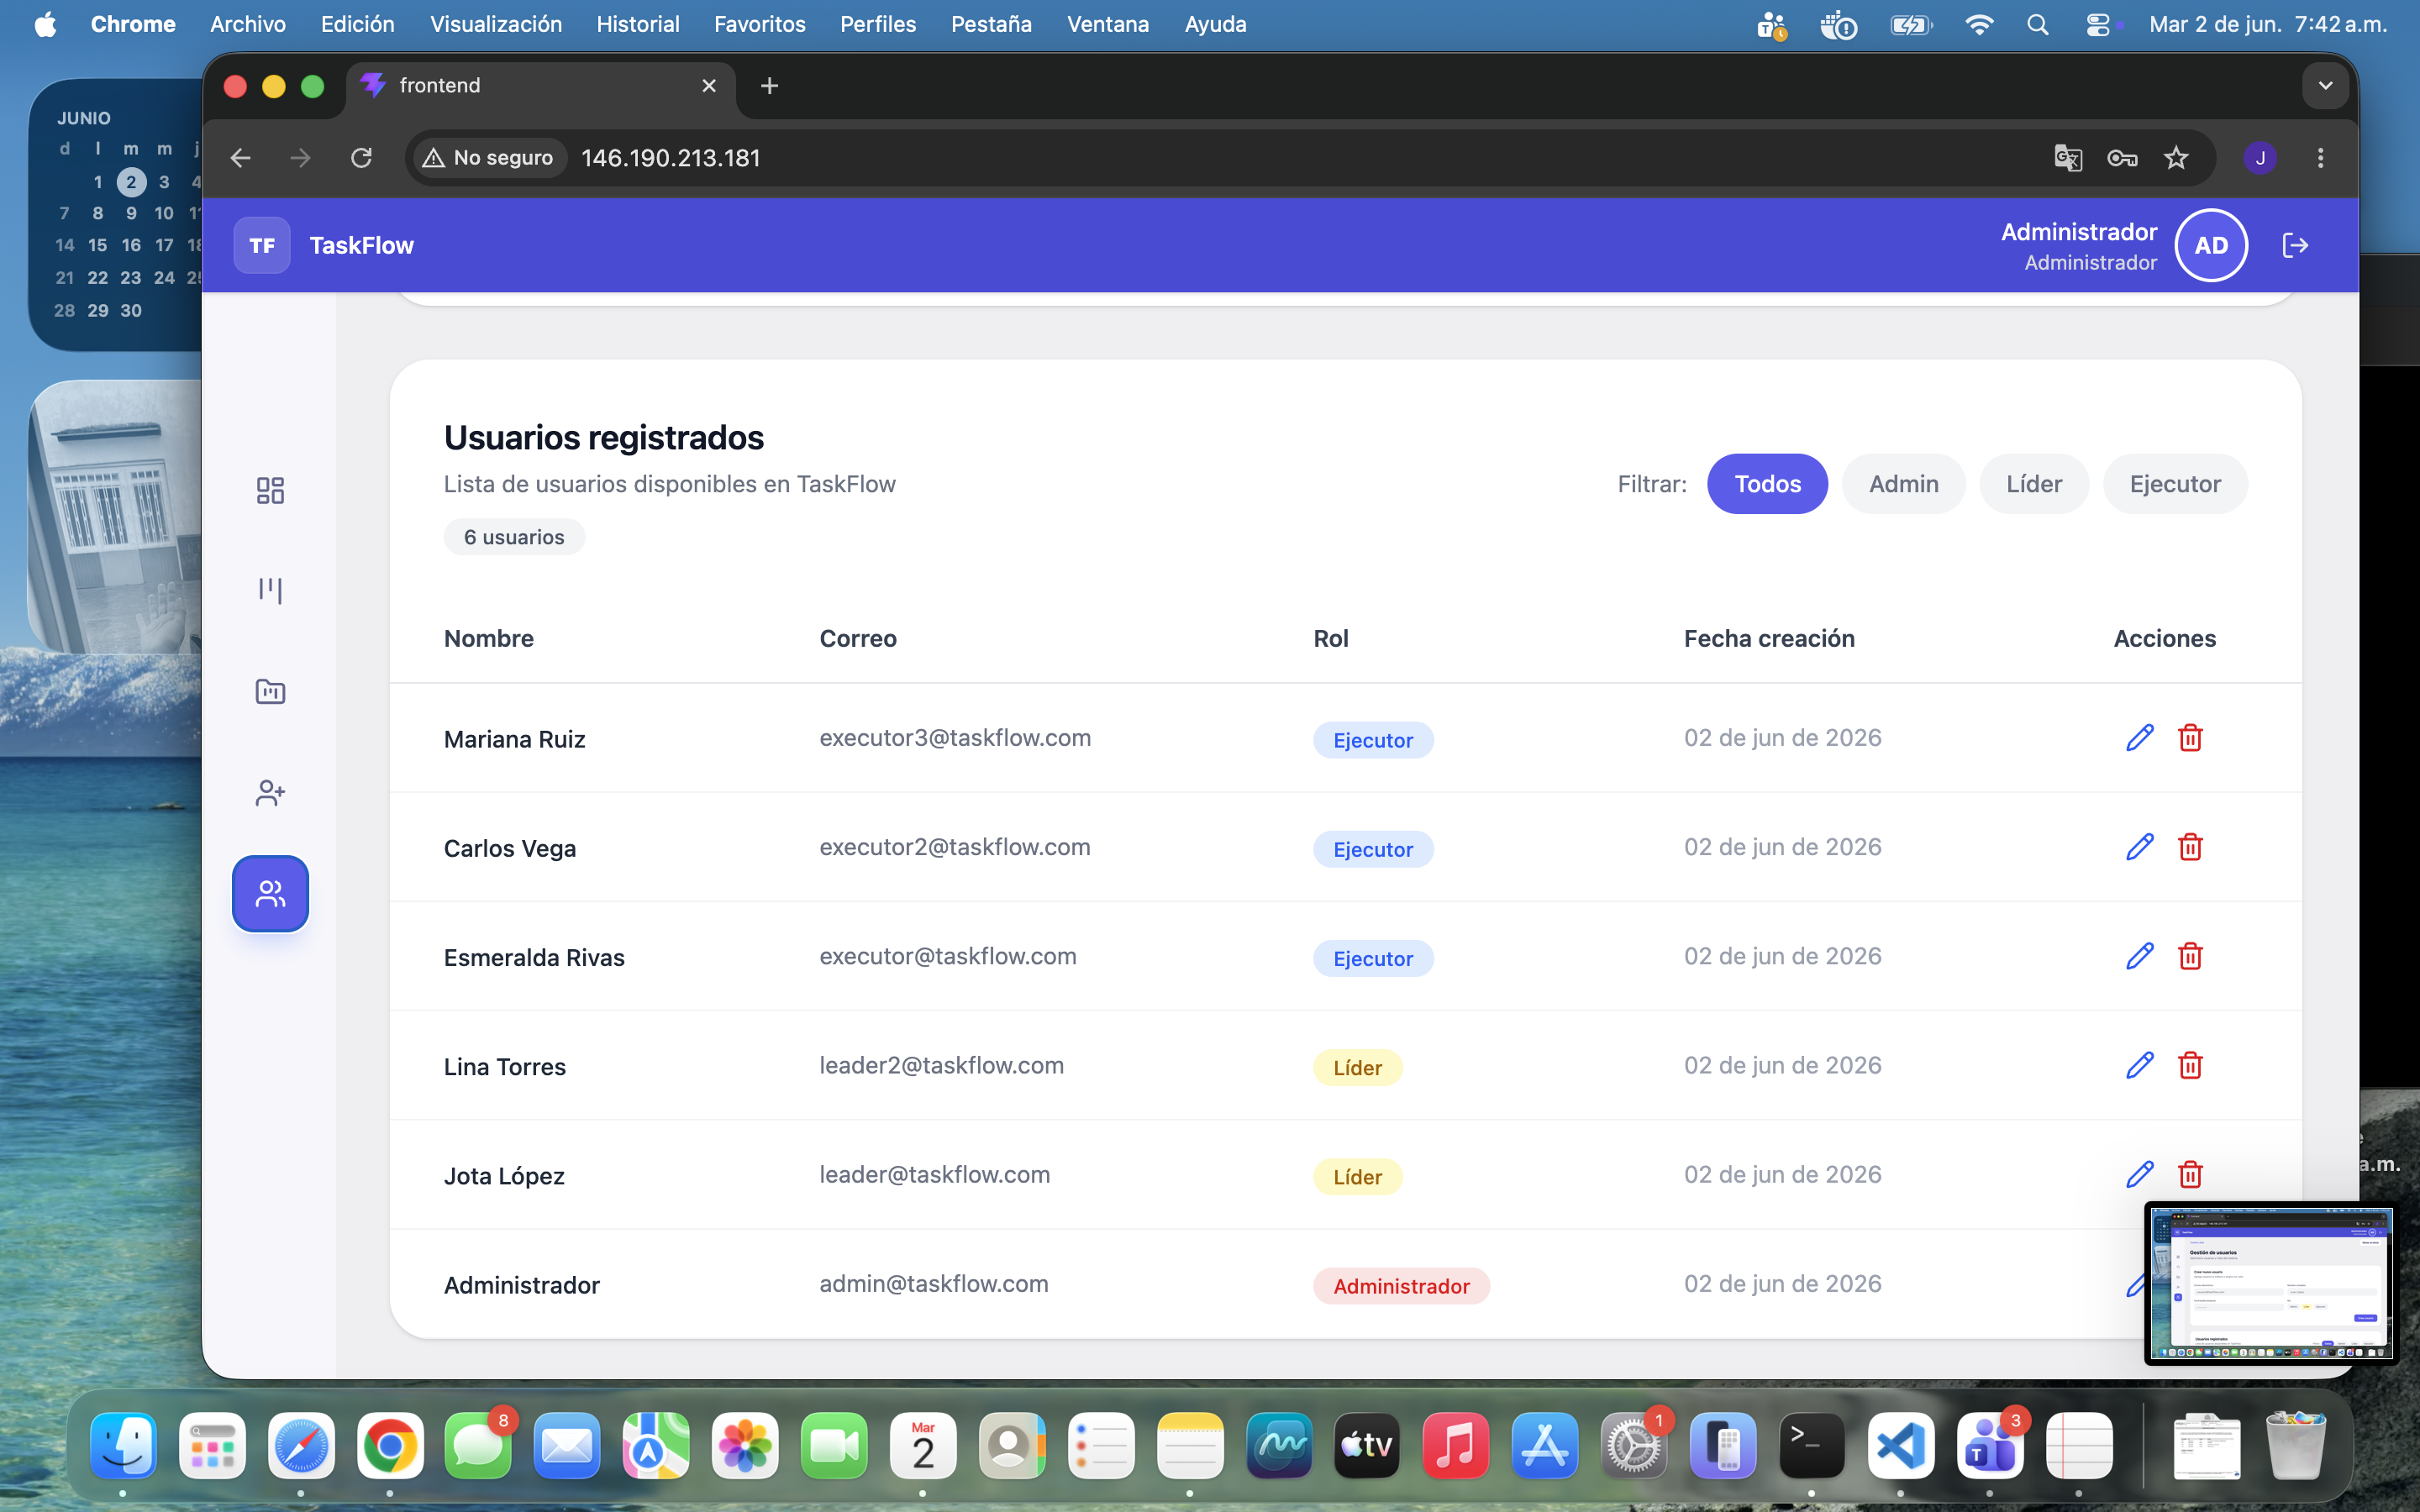
\includegraphics[width=0.90\textwidth]{usuarios-registrados.png}
  \caption{Vista de usuarios registrados en el sistema}
\end{figure}

La tabla de usuarios muestra:
\begin{itemize}
  \item Nombre del usuario.
  \item Correo electrónico.
  \item Rol asignado.
  \item Acciones disponibles (editar, eliminar).
\end{itemize}

% ═══════════════════════════════════════════════════════════════════════════════
\section{Asignación de Personas a Proyectos}

\begin{notebox}
\textbf{Roles con acceso:} \admin\ \leader
\end{notebox}

\subsection{Descripción}

Este módulo permite controlar qué usuarios tienen acceso a cada proyecto, definiendo así quiénes pueden ver el tablero Kanban y ser asignados a sus tareas.

\begin{figure}[H]
  \centering
  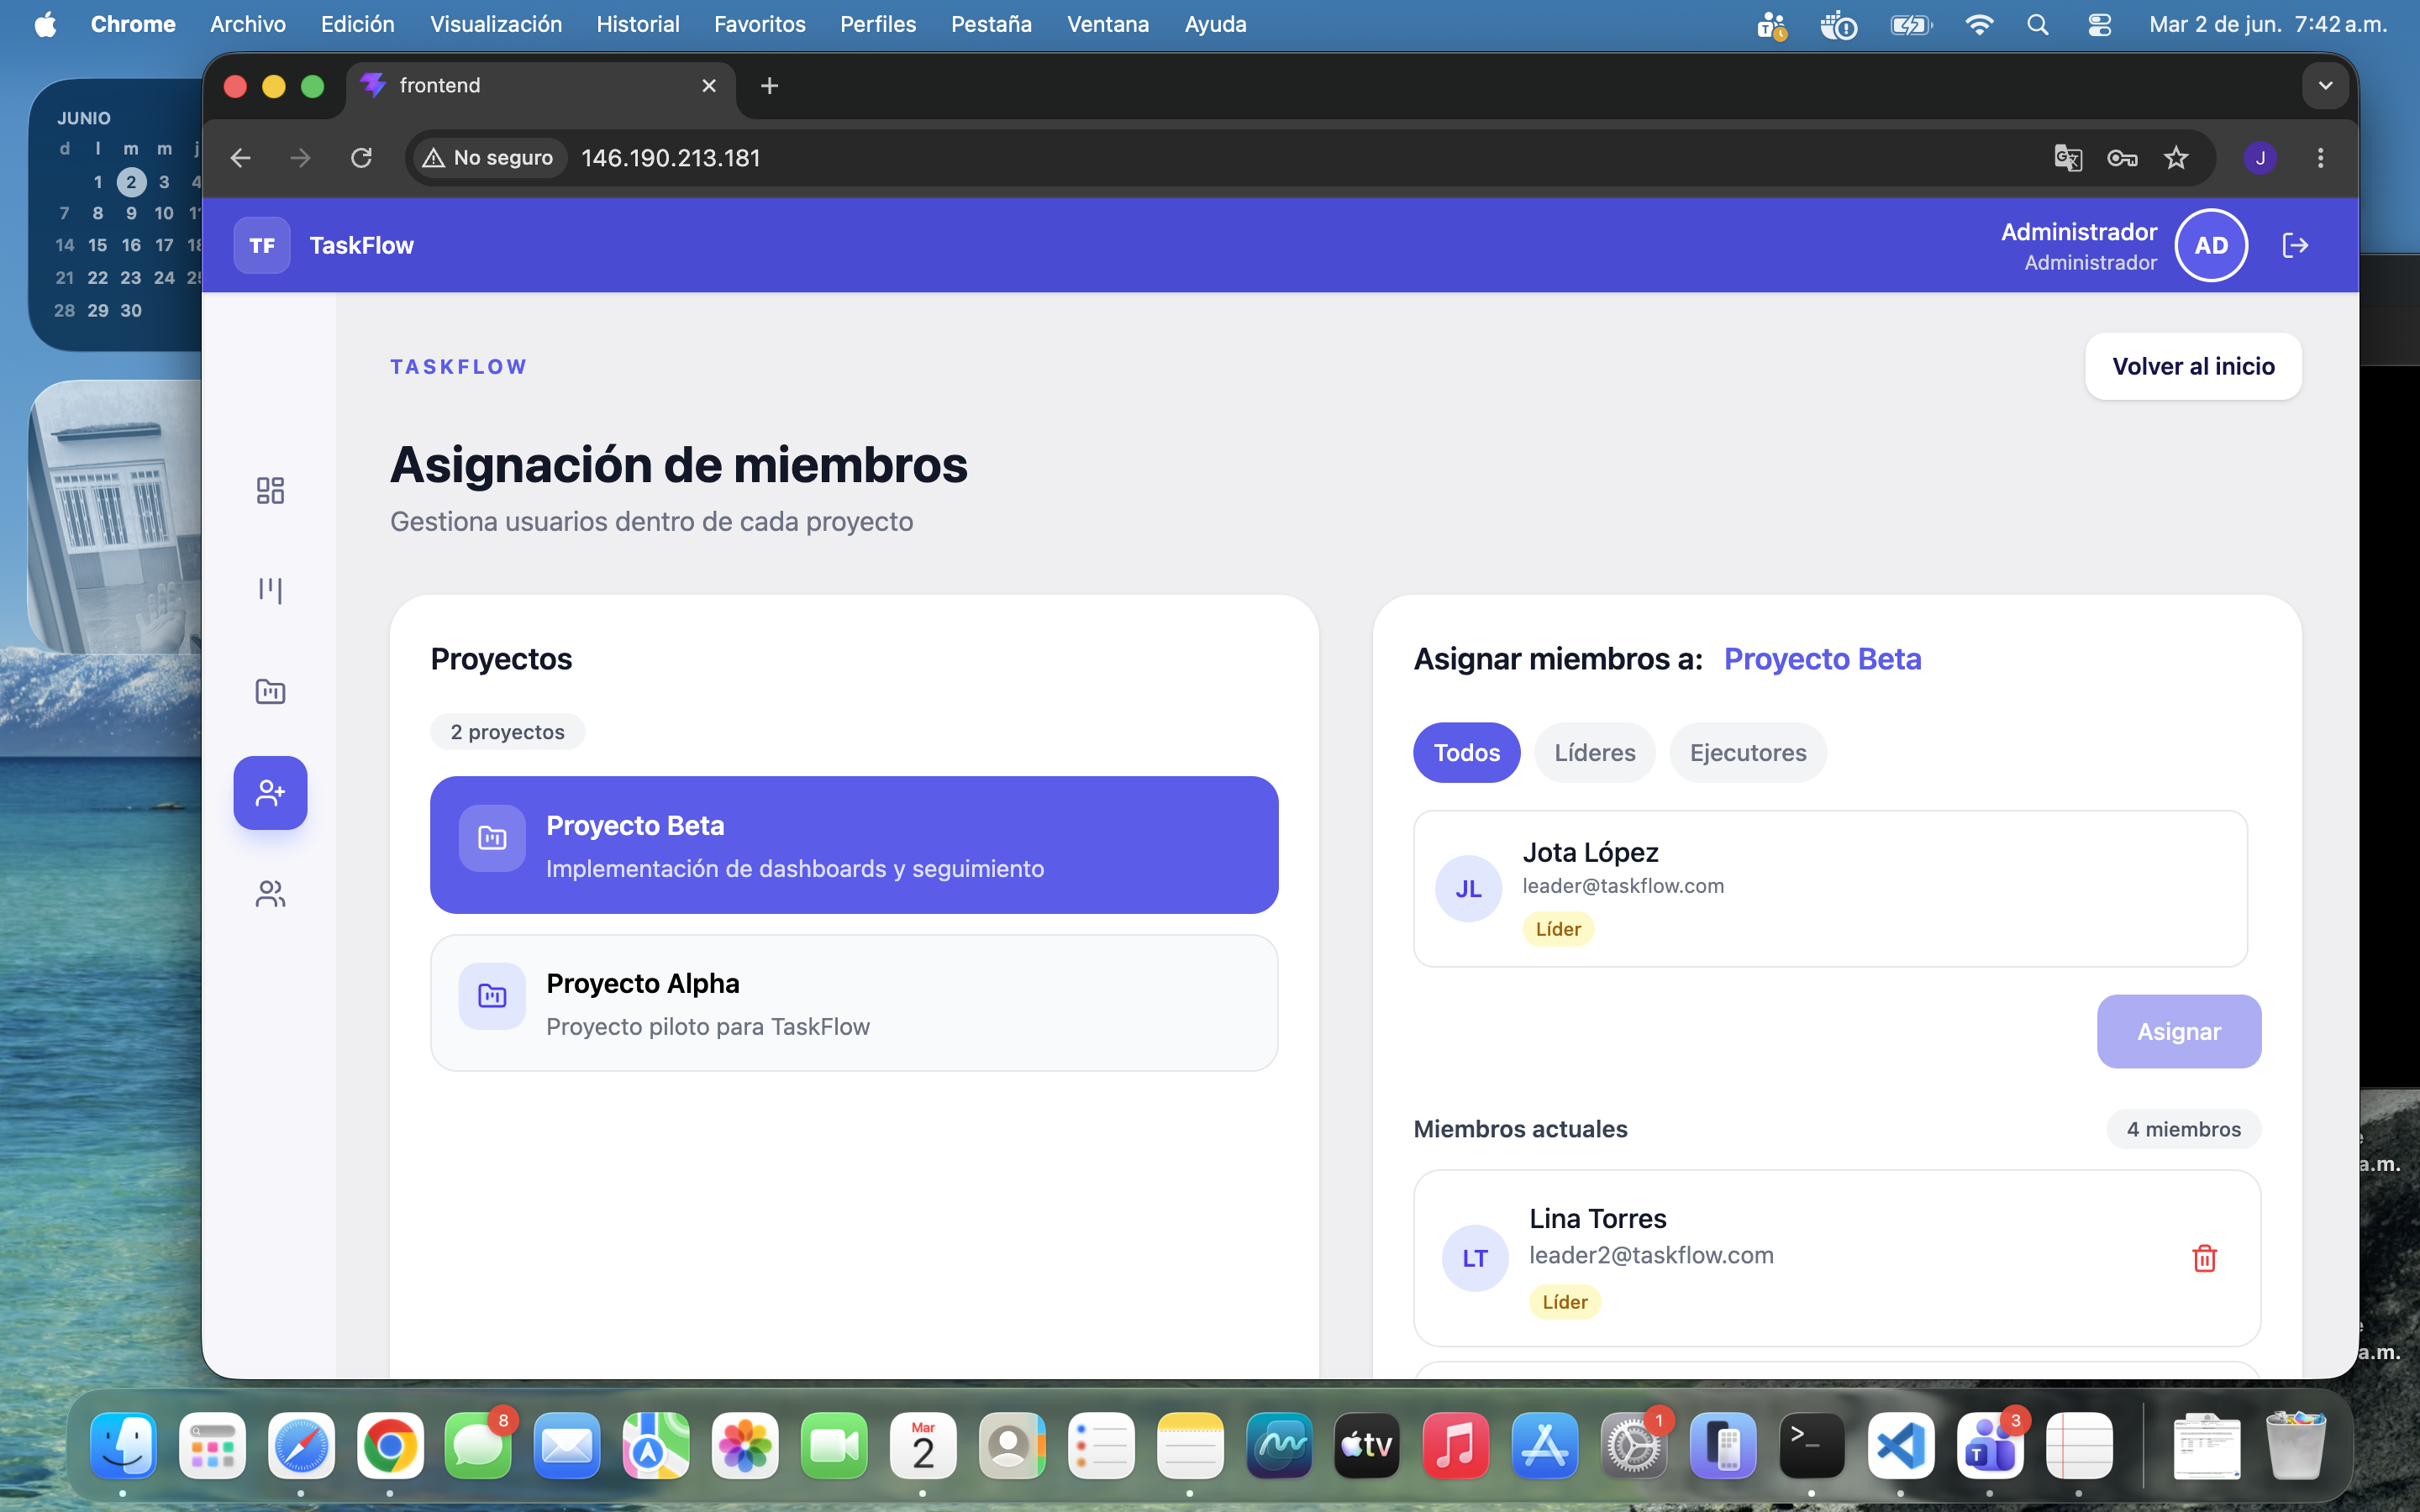
\includegraphics[width=0.90\textwidth]{asignacion-personas.png}
  \caption{Módulo de asignación de miembros al proyecto}
\end{figure}

\subsection{Agregar un miembro}

\begin{enumerate}
  \item Acceda al módulo \textbf{Miembros} desde la barra de navegación.
  \item Seleccione el proyecto al que desea agregar un miembro.
  \item Presione \textbf{«+ Agregar Miembro»}.
  \item Seleccione el usuario de la lista desplegable.
  \item Confirme la asignación.
\end{enumerate}

\begin{infobox}[Asignación del creador]
Al crear un proyecto, su creador queda automáticamente registrado como miembro del mismo.
\end{infobox}

\subsection{Retirar un miembro}

\begin{enumerate}
  \item Localice al miembro en la lista del proyecto.
  \item Presione el ícono de eliminación junto a su nombre.
  \item Confirme la acción.
\end{enumerate}

\begin{warningbox}[Efecto sobre las tareas]
Al retirar a un miembro del proyecto, el sistema desasigna automáticamente todas las tareas que tuviera asignadas dentro de ese proyecto. Dichas tareas quedarán sin responsable y deberán ser reasignadas manualmente.
\end{warningbox}

\subsection{Consultar miembros de un proyecto}

La lista de miembros muestra para cada usuario:
\begin{itemize}
  \item Nombre completo.
  \item Correo electrónico.
  \item Rol en el sistema.
\end{itemize}

% ═══════════════════════════════════════════════════════════════════════════════
\section{Cierre de Sesión}

\subsection{Procedimiento}

Para finalizar la sesión de forma segura:

\begin{enumerate}
  \item Localice el menú de usuario en la barra de navegación (generalmente en la esquina superior derecha o en el menú lateral).
  \item Seleccione la opción \textbf{«Cerrar Sesión»}.
  \item El sistema invalidará la sesión activa.
  \item Será redirigido automáticamente a la pantalla de inicio de sesión.
\end{enumerate}

\subsection{Resultado}

\begin{itemize}
  \item El token de sesión queda eliminado del navegador.
  \item Cualquier intento de acceder a rutas protegidas redirigirá al login.
  \item Para volver a ingresar es necesario autenticarse nuevamente.
\end{itemize}

\begin{infobox}[Buena práctica]
Siempre cierre sesión al finalizar su jornada de trabajo, especialmente si utiliza un equipo compartido. Recuerde que la sesión también expira automáticamente después de 8 horas.
\end{infobox}

% ═══════════════════════════════════════════════════════════════════════════════
\section{Matriz de Permisos}

La siguiente tabla consolida todas las acciones del sistema y los roles habilitados para realizarlas.

\begin{longtable}{L{5.5cm} C{2.2cm} C{2.2cm} C{2.2cm}}
\toprule
\textbf{Acción} & \admin & \leader & \executor \\
\midrule
\endfirsthead
\toprule
\textbf{Acción} & \admin & \leader & \executor \\
\midrule
\endhead
\bottomrule
\endlastfoot

\multicolumn{4}{l}{\textit{\small Usuarios}} \\[2pt]
Crear usuarios                    & \checkmark &            &            \\
Editar nombre / rol de usuario    & \checkmark &            &            \\
Eliminar usuarios                 & \checkmark &            &            \\
\addlinespace
\multicolumn{4}{l}{\textit{\small Proyectos}} \\[2pt]
Crear proyectos                   & \checkmark & \checkmark &            \\
Editar proyectos                  & \checkmark & \checkmark &            \\
Eliminar proyectos                & \checkmark & \checkmark &            \\
Ver todos los proyectos           & \checkmark &            &            \\
Ver proyectos propios             & \checkmark & \checkmark & \checkmark \\
\addlinespace
\multicolumn{4}{l}{\textit{\small Fases}} \\[2pt]
Agregar fases personalizadas      & \checkmark & \checkmark &            \\
Renombrar fases                   & \checkmark & \checkmark &            \\
Eliminar fases                    & \checkmark & \checkmark &            \\
\addlinespace
\multicolumn{4}{l}{\textit{\small Miembros del proyecto}} \\[2pt]
Agregar miembros                  & \checkmark & \checkmark &            \\
Retirar miembros                  & \checkmark & \checkmark &            \\
Ver miembros                      & \checkmark & \checkmark &            \\
\addlinespace
\multicolumn{4}{l}{\textit{\small Tareas}} \\[2pt]
Crear tareas                      & \checkmark & \checkmark &            \\
Editar tareas                     & \checkmark & \checkmark &            \\
Eliminar tareas                   & \checkmark & \checkmark &            \\
Ver tareas del proyecto           & \checkmark & \checkmark & \checkmark \\
Mover tareas entre fases          & \checkmark & \checkmark & \textit{(propias)} \\
Asignar responsable               & \checkmark & \checkmark &            \\
\addlinespace
\multicolumn{4}{l}{\textit{\small Tiempo y comentarios}} \\[2pt]
Registrar tiempo                  & \checkmark & \checkmark & \textit{(propias)} \\
Publicar comentarios              & \checkmark & \checkmark & \checkmark \\
Adjuntar archivos a comentarios   & \checkmark & \checkmark & \checkmark \\
\addlinespace
\multicolumn{4}{l}{\textit{\small Dashboards}} \\[2pt]
Ver resumen del proyecto          & \checkmark & \checkmark & \checkmark \\
Ver carga laboral                 & \checkmark & \checkmark &            \\
\end{longtable}

% ═══════════════════════════════════════════════════════════════════════════════
\section{Recomendaciones de Uso}

\subsection{Para todos los usuarios}

\begin{itemize}
  \item Mantenga actualizadas las tareas asignadas para reflejar el estado real del trabajo.
  \item Registre el tiempo trabajado al finalizar cada sesión de trabajo para mantener métricas precisas.
  \item Utilice los comentarios para documentar avances, dudas o decisiones importantes, seleccionando el tipo de interacción apropiado.
  \item Cierre sesión siempre que termine de usar el sistema, especialmente en equipos compartidos.
\end{itemize}

\subsection{Para administradores y líderes}

\begin{itemize}
  \item Revise periódicamente el dashboard de carga laboral para identificar desequilibrios en el equipo.
  \item Configure fechas de inicio y límite en los proyectos y tareas para facilitar el seguimiento de plazos.
  \item Use fases personalizadas para adaptar el Kanban al flujo de trabajo específico de cada proyecto.
  \item Al retirar a un miembro de un proyecto, verifique que sus tareas hayan sido reasignadas antes de proceder.
\end{itemize}

\subsection{Para ejecutores}

\begin{itemize}
  \item Revise diariamente el tablero Kanban para conocer el estado actualizado de las tareas.
  \item Si una tarea está próxima a vencer, comuníquelo mediante un comentario con interacción \textbf{Duda} o \textbf{Desaprobado} para alertar al líder.
  \item Adjunte evidencias o documentos relevantes a los comentarios para facilitar la revisión por parte del líder del proyecto.
\end{itemize}

% ─── Pie final ───────────────────────────────────────────────────────────────
\vspace{2cm}
\noindent{\color{bordergray}\rule{\textwidth}{0.5pt}}
\begin{center}
  \small\color{medgray}
  \textbf{TaskFlow v1.0} — Manual de Usuario \\
  Jota Emilio Lopez Ramirez y Esmeralda Rivas Guzmán — Junio 2026 \\[2pt]
  Documento sujeto a actualización. Última revisión: junio 2026.
\end{center}

\end{document}
